\documentclass{article}

\usepackage{amsmath}
\usepackage{color}
\usepackage{amssymb}
\usepackage[english]{babel}
\usepackage{graphicx}
\usepackage{listings, multicol}
\usepackage{subfig}
\usepackage{tikz}
\usepackage{hyperref}
\usepackage{makeidx}

\newcommand{\norm}[1]{\lVert#1\rVert}
\newcommand{\vect}[1]{\mathbf{#1}}
\newcommand{\bol}[1]{\boldsymbol{#1}}
\newcommand{\HiFlow}{HiFlow\texorpdfstring{\textsuperscript{3} }{3 }}
\definecolor{lbcolor}{rgb}{0.97,0.97,0.97}

%% Information for PDF-Datei
\hypersetup{
pdfauthor={Ulrich Blunck, Tobias Hahn},
pdftitle={Tutorial Generalized Porous Media Equation},
pdfsubject={Generalized Porous Media Equation},
pdfkeywords={Not set}
}

% Print URLs not in Typewriter Font
\def\UrlFont{\rm}

% Index-Datei öffnen
\makeindex
%%%%%%%%%%%%%%%%%%%%%%%%%%%%%%%%%%%%%%%%%%%%%%
\begin{document}

%Title page
\pagenumbering{roman}
\begin{titlepage}
\def\usesf{}
\let\usesf\sffamily % diese Zeile auskommentieren für normalen TeX Font
\setlength{\unitlength}{1pt}
\Large\bfseries \textsf{\hspace{30pt}Tutorial}
\thispagestyle{empty}\\ 
\noindent\rule{\textwidth}{1pt}
\begin{picture}(0,0)(-250,-25)
\includegraphics[scale=.22]{emcl.pdf} 
\end{picture}

\begin{center}
\hbox{}

{\usesf
\vspace{40pt}
{\normalsize\mdseries U. Blunck, T. Hahn\\}
\vspace{20pt}
{\huge\bfseries Boundary Value Problem for Incompressible Generalized Porous Media Equation\par}
\vspace{20pt}
{\normalsize\mdseries September 20$^\text{th}$, 2012\\}
\vskip 2.5cm

\includegraphics[scale=.4]{HF3_color.png} 

\vspace{-20pt}
\normalsize\mdseries{\hspace{170pt}Version 1.2}
}
\end{center}
\vfill
\noindent\rule{\textwidth}{1pt}
\begin{flushright}
\normalsize\mdseries\textsf{http://www.hiflow3.org\hspace{20pt}}
\end{flushright}
\end{titlepage}

% Contents
\renewcommand{\contentsname}{Contents}
\pagenumbering{Roman}

{\parskip 0pt\tableofcontents} % toc bitte einzeilig



%% ++++++++++++++++++++++++++++++++++++++++++
%% Main part
%% ++++++++++++++++++++++++++++++++++++++++++
\graphicspath{{Bilder/}}

\pagenumbering{arabic}
\renewcommand{\contentsname}{Introduction}

\pagebreak

\fbox{
\begin{minipage}{0.9\linewidth}\vspace*{15pt}\hspace*{15pt}\Large\textbf{Using HiFlow$^\textbf{3}$ for solving the\\\hspace*{15pt}incompressible Generalized Porous\\\hspace*{15pt}Media Equation}\vspace*{15pt}
\end{minipage}
}

\section{Introduction}

HiFlow$^\text{3}$ is a multi-purpose finite element software providing powerful tools for efficient and accurate solution of a wide range of problems modeled by partial differential equations (PDEs). Based on object-oriented concepts and the full capabilities of C++ the HiFlow$^\text{3}$  project follows a modular and generic approach for building efficient parallel numerical solvers. It provides highly capable modules dealing with the mesh setup, finite element spaces, degrees of freedom, linear algebra routines, numerical solvers, and output data for visualization. Parallelism - as the basis for high performance simulations on modern computing systems - is introduced on two levels: coarse-grained parallelism by means of distributed grids and distributed data structures, and fine-grained parallelism by means of platform-optimized linear algebra back-ends.

As the generalized porous media equation presented in this tutorial is closely related to the Navier-Stokes equation, the basic structure and the program have been inherited from the HiFlow\textsuperscript{3} tutorial ``Boundary Value Problem for Incompressible Navier-Stokes
Equation'' by M. Baumann, A. Helfrich-Schkarbanenko, E. Ketelaer, S. Ronn\aa{}s and M. Wlotzka \cite{NSTut}.


\subsection{How to use the Tutorial}

You find the example code (\texttt{porous\_media.cc}, \texttt{porous\_media.h})and a
parameter file (\texttt{porous\_media.xml})\index{configuration file} in the folder
\texttt{/hiflow/examples/porous\_media}. The geometry data (\texttt{*.inp}, \texttt{*.vtu}) is stored in the
folder \texttt{/hiflow/examples/ data}.\index{geometry!folder}



% You can find the example code, data and Makefile in the folder \texttt{/hiflow/examples/porous\_media}. If
% necessary adapt the path in the Makefile, where the library HiFlow$^3$ is installed. The flow tutorial
% must be linked to the library metis (www.cs.umn.edu/$\sim$metis).
% 
% At the current state the stationary GPME can be solved for problems involving 2 or 3 spatial dimensions. To change the number of dimensions, the definition of the \texttt{DIMENSION} variable in the \texttt{porous\_media.h} file (line 31) needs to be adapted accordingly. A detailed derivation of the GPME, as well as additional details regarding its implementation and evaluation can be found in \cite{Blunck}. 

\subsubsection{Using \HiFlow as a Developer}

First build and compile  HiFlow$^\text{3}$ . Go to the directory \texttt{/build/example/porous\_ media}, where the binary generalized porous media equation tutorial is stored. Type \newline\mbox{\textbf{./porous\_media}} to execute the program in sequential mode. You need to make sure that the default parameter file \texttt{porous\_media.xml} is stored in the same directory as the binary, and that the geometry data specified in the parameter file is stored in \texttt{/hiflow/examples/data}.

\pagebreak

\section{Mathematical Setup}
\label{ch:mathSetup}

\subsection{Problem}

We consider the simulation of stationary porous flow in a two-dimensional channel $\Omega$ with narrow in- and outflow. A rectangular obstacle is introduced at the inlet to facilitate spreading of the fluid. 
\vspace{-25pt}
\begin{figure}[!h]
\centering
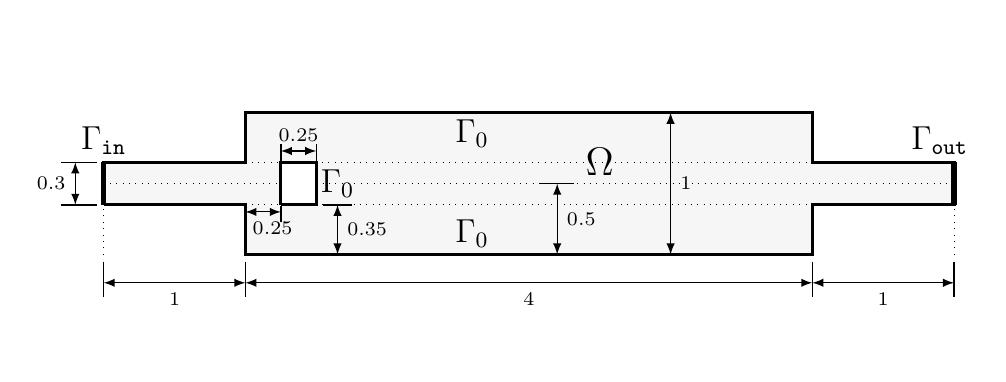
\begin{tikzpicture}[scale=1.8]
\tikzstyle{every node}=[font=\small]
%exterior nodes
\path (0,1.6cm) coordinate (v0);
\path (0,-.7cm) coordinate (v0);
\path (0,.35cm) coordinate (v0);
\path (1,.35cm) coordinate (v1);
\path (1,0cm) coordinate (v2);
\path (5,0cm) coordinate (v3);
\path (5,.35cm) coordinate (v4);
\path (6,.35cm) coordinate (v5);
\path (0,.65cm) coordinate (v6);
\path (1,.65cm) coordinate (v7);
\path (1,1cm) coordinate (v8);
\path (5,1cm) coordinate (v9);
\path (5,.65cm) coordinate (v10);
\path (6,.65cm) coordinate (v11);
%Interior Nodes
\path (1.25,.35cm) coordinate (b0);
\path (1.5,.35cm) coordinate (b1);
\path (1.5,.65cm) coordinate (b2);
\path (1.25,.65cm) coordinate (b3);
%outline/inline
\draw [line width=1pt,fill=gray!7] (v0) -- (v1) -- (v2) -- (v3) -- (v4) -- (v5) -- (v11) -- (v10) -- (v9) -- (v8) -- (v7) -- (v6) -- (v0);
\draw [line width=1pt, fill=white] (b0) -- (b1) -- (b2) -- (b3) -- (b0);


%Distance Arrows
\draw [latex-latex,line width=.4pt] (0,-.2) -- node[below] {\scriptsize$1$} (1,-.2);  
\draw [latex-latex,line width=.4pt] (1,-.2) -- node[below] {\scriptsize$4$} (5,-.2);
\draw [latex-latex,line width=.4pt] (5,-.2) -- node[below] {\scriptsize$1$} (6,-.2);
\draw [latex-latex,line width=.4pt] (-.2,.35) -- node[left] {\scriptsize$0.3$} (-.2,.65);
\draw [latex-latex,line width=.4pt] (4,0) -- node[right] {\scriptsize$1$} (4,1);
\draw [latex-latex,line width=.4pt] (3.2,0) -- node[right] {\scriptsize$0.5$} (3.2,.5);
\draw [latex-latex,line width=.4pt] (1,.3) -- node[below, font=\scriptsize ] {$\;\;\;$\scriptsize$0.25$} (1.25,.3);
\draw [latex-latex,line width=.4pt] (1.65,.35) -- node[right,font=\scriptsize ] {\scriptsize$0.35$} (1.65,0);
\draw [latex-latex,line width=.4pt] (1.25,.73) -- node[above,font=\scriptsize ] {\scriptsize$0.25$} (1.5,.73);

%Border Arrows
\draw [-,line width=.5pt] (0,-.05) -- (0,-.3);
\draw [-,line width=.5pt] (1,-.05) -- (1,-.3);
\draw [-,line width=.5pt] (5,-.05) -- (5,-.3);
\draw [-,line width=.5pt] (6,-.05) -- (6,-.3);
\draw [-,line width=.5pt] (-.05,.35) -- (-.3,.35);
\draw [-,line width=.5pt] (-.05,.65) -- (-.3,.65);
\draw [-,line width=.5pt] (3.08,.5) -- (3.32,.5);
\draw [-,line width=.5pt] (1.25,.34) -- (1.25,.23);
\draw [-,line width=.5pt] (1.55,.35) -- (1.75,.35);
\draw [-,line width=.5pt] (1.25,.66) -- (1.25,.78);
\draw [-,line width=.5pt] (1.5,.66) -- (1.5,.78);

%dotted lines
\draw [dotted,line width=.3pt] (0,.5) -- (1.25,.5);
\draw [dotted,line width=.3pt] (1.5,.5) -- (6,.5);
\draw [dotted,line width=.3pt] (1,.35) -- (5,.35);
\draw [dotted,line width=.3pt] (1,.65) -- (5,.65);
\draw [dotted,line width=.3pt] (0,0) -- (0,.35);
\draw [dotted,line width=.3pt] (6,0) -- (6,.35);

\draw [line width=2pt] (v5) -- (v11);
\draw [line width=2pt] (v0) -- (v6);

\node [font=\large] at (3.5,.65) {\Large$\Omega$};
\node [font=\normalsize] at (1.65,.5) {\large$\Gamma_0$};
\node [font=\normalsize] at (2.6,.15) {\large$\Gamma_0$};
\node [font=\normalsize] at (2.6,.85) {\large$\Gamma_0$};
\node [font=\large] at (-.,.8) {\large$\Gamma_{\texttt{in}}$};
\node [font=\large] at (5.9,.8) {\large$\Gamma_{\texttt{out}}$};
\end{tikzpicture}

\vspace{-20pt}
\caption{Non-dimensional ratio of the measurements used for the geometry.}
\label{fig:geomnodim}
\end{figure}\index{geometry}

% \vspace{-10pt}
The liquid is assumed to be an incompressible Newtonian fluid\index{Newtonian fluid}. The porous medium is assumed to be uniformly distributed with well connected vacancies for each respective subdomain. The size of the single components of the porous medium, as well as the size of the vacancies, is assumed to be significantly smaller than the modeled domain. Thus, the fluid flow within the column can be modeled using the Generalized Porous Media Equation  \cite{Blunck}, see \eqref{eqn:red1}.\\
There are three different boundary conditions\index{boundary conditions} to be distinguished:

\vspace*{10pt}\hspace*{20pt} The inflow condition at the inflow $\Gamma_{\texttt{in}}$, see \eqref{eqn:bound1}.\\
\hspace*{20pt} The outflow condition at the exit $\Gamma_{\texttt{out}}$, see \eqref{eqn:bound2}.\\
``No-Slip'' condition at the remaining boundaries $\Gamma_{\texttt{0}}(=\partial \Omega \backslash \overline{(\Gamma_{\texttt{in}} \cup \Gamma_{\texttt{out}})}\,)$, \eqref{eqn:bound3}. 

\vspace*{10pt}
At the outflow, the natural Neumann- (so called ``Do-Nothing''-) condition\index{boundary conditions!Neumann}, adapted to porous flow, is applied. On both of the remaining two boundaries, Dirichlet\index{boundary conditions!Dirichlet} boundary conditions are used.\\
In the formulation of the GPME used in this tutorial, the external body forces\index{external body forces} are neglected.\\
These premises lead to the following boundary value problem for the unknown velocity field $\vect u=(u_1,u_2)^\top$\index{velocity} and the pressure field $p$\index{pressure} (with each $u_1$, $u_2$ and $p$ being functions of $(x_1,x_2)^\top$):

\begin{subequations}
 \begin{eqnarray}
\!\!\!\!\!\!\!\!\!\!\!\!\!\!\!\!\!\!\frac{1}{\varepsilon} \left(\vect u \cdot \nabla \right) \frac{\vect u}{\varepsilon}  + \frac{1}{\varepsilon {\varrho_f}} {\nabla p \, \varepsilon} + \frac{{\nu_e}}{\varepsilon} \Delta \vect u  + \frac{\nu_f }{\kappa}\vect u + \frac{1.75}{\sqrt{150}} \frac{1}{\sqrt{\kappa}} \frac{\norm{\vect u}}{\varepsilon^{3/2}}\vect u &=\, \vect 0 &\text{  in $\Omega$} \label{eqn:red1}\\
    \nabla \cdot \vect u&=\,0 &\text{  in $\Omega$} \label{eqn:red2}\\
    \vect u &=\, \vect g &\text{  on $\Gamma_{\texttt{in}}$} \label{eqn:bound1}\\
   (- \bol{\mathcal{I}}p + \frac{\nu_e}{\varepsilon}\nabla \vect u)\cdot \vect n &= \,0 &\text{  on $\Gamma_{\texttt{out}}$}\label{eqn:bound2}\\
  \vect u &=\,\vect 0 &\text{  on $\Gamma_0$}\label{eqn:bound3}
 \end{eqnarray}
\label{eqn:boundaryreduced}
\end{subequations}\index{generalized porous media equation}

The porosity $\varepsilon$\index{porosity} is defined as the ratio $\frac{V_{free}}{V_{ref}}$ of the interstitial volume $V_{free}$ to the absolute one $V_{ref}$ of a reference volume and is assumed to behave locally constant. Same holds for the permeability\index{permeability} $\kappa$, which is specific to the utilized porous media. The density\index{density} of the fluid ${\varrho_f}$ is constant in the domain, as only incompressible fluids are considered. The effective kinematic viscosity\index{kinematic viscosity!effective} of the fluid within the porous medium $\nu_e$ is assumed to be equal to the kinematic viscosity\index{kinematic viscosity} of the fluid itself $\nu_f$ \cite[p. 356]{Viscosity}, which is a fluid-specific constant. The vector $\vect n=\vect (n_1,n_2)^{\top}$ (with each component dependent on $(x_1,x_2)^{\top}$) denotes the outer normal vector on $\partial \Omega$ and $\boldsymbol{\mathcal{I}} \in \mathbb{R} ^ {2 \times 2}$ the unit matrix. The flow profile\index{flow profile} described by the given function $\vect g:\Gamma_{\texttt{in}} \rightarrow \mathbb{R}^2$ is enforced at the inflow.

\subsection{Solving the non-linear problem with Newton's method}

Due to the terms accounting for the convective acceleration\index{convective acceleration} $\left(\frac{1}{\varepsilon} \left(\vect u \cdot \nabla \right) \frac{\vect u}{\varepsilon}\right)$ and the non-linear drag contribution\index{drag term!non-linear} $\left(\frac{1.75}{\sqrt{150}} \frac{1}{\sqrt{\kappa}} \frac{\norm{\vect u}}{\varepsilon^{3/2}}\vect u\right)$\,, the Generalized Porous Media Equation \eqref{eqn:red1} is a non-linear equation. One possibility to solve a non-linear problem is using iterative Newton’s method\index{Newton's method}, which in general is a method to find the zero of a function $F$, i.e.

\begin{equation*}
 F(\bol \xi)=0,
\end{equation*}

 where $\bol \xi=(\vect u,p)^{\top}$ represents the solution. The corresponding Newton-Iteration has the form:

\begin{equation*}
\quad\qquad\qquad \bol \xi ^ {k+1} := \bol \xi ^ {k} - \underbrace{(\nabla F (\bol \xi ^ {k})) ^ {-1}F(\bol \xi ^{k})}_{ \vect c^k} \;,\quad\quad k=0,1,2,\dots
\label{eqn:Newton} 
\end{equation*}

Or, avoiding the necessity of deriving of the inverse of $\nabla F (\bol \xi ^ {k})$, the iteration can be written as:

\begin{equation}\label{eqn:NewtonApp}
\qquad\qquad\qquad\qquad \left.\begin{aligned}
        \nabla F (\bol \xi ^ {k}) \, \vect c^k &= F (\bol \xi ^k) \\
        \bol \xi ^ {k+1} &= \bol \xi ^{k} - \vect c^k 
       \end{aligned}
 \right. \qquad\qquad k=0,1,2,\dots
\end{equation}
The vector $\vect c^k =(\vect c_u^k,c_p^k)^{\top}$ denotes the correction term\index{correction term} of the $k\,$th iteration step. The start solution $\bol \xi^0$ is given.The term $\nabla F(\bol \xi^k)\,\vect c^k$ denotes the linearization\index{linearization}, which is the derivative of $F$ at the linearization point $\bol \xi^k$ in the direction
$\vect c^k$. For the GPME the function $F$ is defined via \eqref{eqn:red1},\eqref{eqn:red2} as:

\begin{align}\label{eqn:Feq}
F(\vect u^k,p^k) &\!:=
\begin{pmatrix}
F_1(\vect u^k,p^k)\\
F_2(\vect u^k,p^k)
\end{pmatrix} \nonumber \\
&\,=
\begin{pmatrix}
\frac{1}{\varepsilon} \left( \vect u^k \cdot \nabla \right) \frac{ \vect u^k}{\varepsilon}  + \frac{1}{\varepsilon{\varrho_f}} {\nabla p^k \varepsilon} - \frac{{\nu_e}}{\varepsilon} \Delta  \vect u^k  + \frac{\nu_f  }{\kappa}\vect u^k + \frac{1.75}{\sqrt{150}} \frac{1}{\sqrt{\kappa}} \frac{\norm{\vect u^k}}{\varepsilon^{3/2}} \vect u^k\\
\nabla \cdot  \vect u^k
\end{pmatrix}.
\end{align}

The derivation of the linearization of the linear terms of \eqref{eqn:Feq} is trivial. Therefore it is only shown here for the non-linear terms\index{non-linear terms!linearization} $\mathcal{N}_1(\vect u):=\frac{1}{\varepsilon} \left(\vect u \cdot \nabla \right) \frac{\vect u}{\varepsilon}$ and $\mathcal{N}_2(\vect u):= \frac{1.75}{\sqrt{150}} \frac{1}{\sqrt{\kappa}} \frac{\norm{\vect u}}{\varepsilon^{3/2}}\vect u$ (index $k$ is omitted for simplicity):
\begin{align*}
 \textstyle{ \nabla_{\vect u} \; \mathcal{N}_1({\vect u})\cdot \vect c_u  }& \textstyle{=\lim_{\lambda \to 0} \frac{1}{\lambda}\left(\mathcal{N}_1(\vect u+\lambda \vect c_u) - \mathcal{N}_1(\vect u)  \right)  }\\
 & \textstyle{= \frac{1}{\varepsilon} \lim_{\lambda \to 0} \frac{1}{\lambda}\big[         \left( (\vect u+\lambda \vect c_u) \cdot \nabla \right) \frac{ (\vect u + \lambda \vect c_u)}{\varepsilon} - \left( {\vect u} \cdot \nabla \right) \frac{{\vect u}}{\varepsilon}  \big] } \\
 & \textstyle{=\frac{1}{\varepsilon} \lim_{\lambda \to 0} \frac{1}{\lambda}\big[    (\vect u \cdot \nabla) \frac{ (\vect u + \lambda \vect c_u)}{\varepsilon} + (\lambda \vect c_u \cdot \nabla) \frac{ (\vect u + \lambda \vect c_u)}{\varepsilon} - \left( {\vect u} \cdot \nabla \right) \frac{{\vect u}}{\varepsilon}  \big] } \\
 & \textstyle{= \frac{1}{\varepsilon} \lim_{\lambda \to 0} \frac{1}{\lambda}\big[    (\vect u \cdot \nabla) \frac{ {\vect u}}{\varepsilon} + (\vect u \cdot \nabla) \frac{ \lambda \vect c_u}{\varepsilon} + (\lambda \vect c_u \cdot \nabla) \frac{{\vect u}}{\varepsilon} }\\
  &\;\;\;\;\;\;\;\;\;\;\;\;\;\;\;\;\;\;\;\;\;\textstyle{ +  (\lambda \vect c_u \cdot \nabla) \frac{ \lambda \vect c_u}{\varepsilon} - \left( {\vect u} \cdot \nabla \right) \frac{{\vect u}}{\varepsilon}  \big]} \\
 & \textstyle{= \frac{1}{\varepsilon} \lim_{\lambda \to 0} \big[  (\vect u \cdot \nabla) \frac{ \vect c_u}{\varepsilon} + ( \vect c_u \cdot \nabla) \frac{{\vect u}}{\varepsilon} + (\vect c_u \cdot \nabla) \frac{ \lambda \vect c_u}{\varepsilon}  \big]  }\\
 &\textstyle{= \frac{1}{\varepsilon}  (\vect u \cdot \nabla) \frac{ \vect c_u}{\varepsilon} + \frac{1}{\varepsilon} ( \vect c_u \cdot \nabla) \frac{{\vect u}}{\varepsilon}  }
\end{align*}

The linearization of term $\mathcal N_2$, the non-linear drag term, requires special attention, as the absolute value of $\vect {u}$ leads to non-differential behavior at $\vect u= \vect 0$. For sake of brevity, the coefficient of the term is summarized in the constant $C$.

\begin{align*}
 { \nabla_{\vect u} \; \mathcal{N}_2(\vect u)\cdot \vect c_u  }& {=\lim_{\lambda \to 0} \frac{1}{\lambda}\left(\mathcal{N}_2(\vect u+\lambda \vect c_u) - \mathcal{N}_2(\vect u)  \right)  }\\
 & {= C  \lim_{\lambda \to 0} \frac{1}{\lambda}\big[    \norm{{\vect u}+\lambda \vect c_u} (\vect u+\lambda \vect c_u) - \norm{{\vect u}}{\vect u} \big] } \\
 & {= C  \lim_{\lambda \to 0} \frac{1}{\lambda}\big[\norm{{\vect u}+\lambda \vect c_u} \vect u+\lambda \norm{{\vect u}+\lambda \vect c_u} \vect c_u - \norm{{\vect u}}{\vect u} \big] }\\
\intertext{Note that the change of each component of the velocity field will influence the value of the non-linear drag term in each other component as well. This poses a great problem, as exact accounting for this correlation is not possible within a linear system and even approximation would largely increase the population of the system matrix.}
\intertext{However, as the influence of the non-linear drag term is only expected to be prominent for very specific parameter combinations, the value of $\norm{{\vect u}+\lambda {\vect c}_u}$ will be approximated using only the values of the velocity field ${\vect u}$ of the previous iteration step.}
 { \nabla_{\vect u} \; \mathcal{N}_2(\vect u)\cdot \vect c_u  }& {\approx C  \lim_{\lambda \to 0} \frac{1}{\lambda}\big[    \norm{{\vect u}}\vect u + \lambda \norm{{\vect u}} \vect c_u - \norm{{\vect u}}{\vect u} \big] } \\
 & {= C  \lim_{\lambda \to 0} \big[    \norm{{\vect u}} ( \vect c_u) \big] } \\
 & {= \frac{1.75}{\sqrt{150}} \frac{1}{\sqrt{\kappa}} \frac{\norm{{{\vect u}}}}{\varepsilon^{3/2}} \vect c_u  }
\end{align*}

The linearization of $F$ is then given by:

\begin{align} \label{eqn:linFeqconst}
\nabla F(\vect u^k,p^k) \cdot \begin{pmatrix} \vect c_u \\ c_p \end{pmatrix}  = \begin{pmatrix}
                                                                          \nabla F_{1}(\bol \xi^k)\\
                                                                          \nabla F_{2}(\bol \xi^k)
                                                                   \end{pmatrix} \cdot \begin{pmatrix} \vect c_u \\ c_p \end{pmatrix} 
\end{align}

with
\begin{align*}
\nabla F_{1}(\bol \xi^k)\cdot \begin{pmatrix} \vect c_u \\ c_p \end{pmatrix}
 =\,& \frac{1}{\varepsilon}  (\vect u^k \cdot \nabla) \frac{ \vect c_u}{\varepsilon} + \frac{1}{\varepsilon} ( \vect c_u \cdot \nabla) \frac{ \vect u^k}{\varepsilon}
 + \frac{1}{{\varrho_f}\,\epsilon} {\nabla c_p \epsilon}                                             
 - \frac{{\nu_e}}{\varepsilon} \Delta  \vect c_u \nonumber \\   
 &\!\!+ \frac{\nu}{\kappa} \vect c_u  
 + \frac{1.75}{\sqrt{150}} \frac{1}{\sqrt{\kappa}} \frac{\norm{{\vect u^k}}}{\varepsilon^{3/2}} \vect c_u                                                            
\intertext{and}
\nabla F_{2}(\bol \xi^k)\cdot \begin{pmatrix} \vect c_u \\ c_p \end{pmatrix}=\,&  \nabla \cdot  \vect c_u .
\end{align*}

To retain the boundary conditions postulated by equations \eqref{eqn:bound1} to \eqref{eqn:bound3}, each correction term $(\vect c_u,c_p)^{\top}$ has to satisfy 

\begin{align*} 
\vect c_u &= \vect 0  &&\text{on $\Gamma_{\texttt{in}}$}\\
\qquad\qquad(-\bol{\mathcal{I}} c_p + \frac{\nu_e}{\varepsilon} \nabla \vect c_u) \cdot \vect n &= 0 &&\text{on $\Gamma_{\texttt{out}}$}\\
\vect c_u &=\vect 0 &&\text{on $\Gamma_{0}$}\;.
\end{align*}

\subsection{Weak Formulation}

To solve a problem using finite element methods, a variational formulation\index{weak formulation} of the problem must be given. It can be derived by multiplying the equation with some test functions\index{test functions}, integrating over the domain, applying integration by parts and the Gauss theorem. Therefore the domain $\Omega$ has to be a Lipschitz domain \cite{Lipschitz}.\\
The solution space\index{solution space} for the velocity $\vect u$ is defined as

\begin{align}
 \mathcal{U}(\Omega) &:= \{\vect u : \vect u \in  H^1 (\Omega)^2, \;\vect u|_{\Gamma_{\texttt{in}}}=\vect g, \; \vect u|_{\Gamma_0}=\vect 0\}
\label{eqn:U_space}\\ \nonumber \\
\intertext{And the corresponding spaces of the velocity and pressure component of the correction term are defined as:}
 \mathcal{V}_u(\Omega) &:= \{\vect u : \vect u \in  {H}^1 (\Omega)^2, \; \vect u|_{\Gamma_{\texttt{in}}\cup\Gamma_0}=\vect 0\}
\label{eqn:Vu_space} \\ \nonumber\\
\mathcal{V}_p(\Omega)&:=\{p : p\in {L}^2(\Omega)\},
\end{align}

Where $L^2$ is the Lebesgue\footnote{Henri León Lebesgue, ($\ast$ 1875, $\dag$ 1941)} space of equivalence classes of square integrable functions in $\Omega$ and $H^1$ the Sobolev\footnote{Sergei Lvovich Sobolev, ($\ast$ 1908, $\dag$ 1989)} space of equivalence classes of square integrable functions with square integrable (weak) first-derivatives in $\Omega$.

The single utilized functions are elements of these function spaces as follows:

$$p,c_p\in \mathcal{V}_p, \quad \vect c_u\in \mathcal{V}_u, \quad \vect u\in \mathcal{U}.$$

The indices $k$ of the single functions have been omitted.

In each Newton step \eqref{eqn:NewtonApp} a problem of the following form has to be solved:

\subsubsection*{Problem}


\fcolorbox{black}{lbcolor}{\parbox{0.97\columnwidth}{
Find $\vect c = (\vect c_u,c_p)^{\top}$ with $\vect c_u\in \mathcal{V}_u$ and $c_p \in \mathcal{V}_p$ such that

 \begin{eqnarray}
 \int_\Omega \nabla F_1 (\bol \xi ^ {k})\, \vect c \circ \vect v \,\mathrm{d}\vect x  =& \displaystyle{\int_\Omega F_1 (\bol \xi ^k) \circ \vect v \,\mathrm{d}\vect x}\nonumber\\\label{eqn:var_grund}
\\
 \int_\Omega \nabla F_2 (\bol \xi ^ {k})\, \vect c \, q \,\mathrm{d}\vect x  =&  \displaystyle{\int_\Omega F_2 (\bol \xi ^k) \,q \,\mathrm{d}\vect x} \nonumber
\end{eqnarray}

for all test functions $\vect v \in \mathcal{V}_u(\Omega)$ and $q\in\mathcal{V}_p(\Omega)$, where $\circ$ denotes multiplication by components.}}
\vspace{0.3cm}\\
The application of the Gauss theorem mentioned above, leads to a formulation of the left-hand side of the equation:

\begin{subequations}
\begin{align*}
  &\int_\Omega \nabla F_1 (\bol \xi ^ {k}) \vect c \circ \vect v \,\mathrm{d}\vect x \nonumber \\
&\hspace{1cm}
\begin{array}{l}
\displaystyle
=\int_\Omega \frac{1}{\varepsilon^2}(\vect u^k \cdot \nabla) \, \vect c_u \circ \vect v
+\frac{1}{\varepsilon^2}( \vect c_u \cdot \nabla) \vect u^k \circ \vect v
+\frac{\nu}{\kappa} \vect c_u \circ \vect v 
- \frac{1}{{\varrho_f}}c_p (\nabla  \circ \vect v) \\ \vspace*{20pt}
\displaystyle\;\;\;\;
+\frac{1.75}{\sqrt{150}} \frac{1}{\sqrt{\kappa}} \frac{1}{\varepsilon^{3/2}}\norm{{\vect u^k}}\vect c_u  \circ \vect v                                                                                      
 +  \frac{{\nu_e}}{\varepsilon}\nabla  \vect c_u : \nabla \vect v  \;\mathrm{d}\vect x
\end{array}
\intertext{and}
& \int_\Omega \nabla F_2 (\bol \xi ^ {k}) \vect c \, q \,\mathrm{d}\vect x \; = 
\begin{array}{l}
\displaystyle
\int_\Omega (\nabla \cdot \vect c_u)q \,\mathrm{d}\vect x .
\end{array}
\end{align*}
\end{subequations}

For the right-hand side the analogous terms
\begin{subequations}
\begin{align*}
&\begin{array}{l}\displaystyle\int_\Omega F_1 (\bol \xi ^ {k}) \circ \vect v \,\mathrm{d}\vect x \;\;\;= \\ \; \\ \; \end{array}
\begin{array}{l}
\displaystyle
\int_\Omega \frac{1}{\varepsilon^2} \left(\vect u^k \cdot \nabla \right) \vect u^k\circ \vect v+\frac{\nu}{\kappa} \vect u^k \circ \vect v - \frac{1}{{\varrho_f}}p (\nabla  \circ \vect v) \\
\displaystyle\;\;\;\;
+\frac{1.75}{\sqrt{150}} \frac{1}{\sqrt{\kappa}} \frac{1}{\varepsilon^{3/2}}\norm{{\vect u^k}}\vect u^k  \circ \vect v                                                                                      
 +  \frac{{\nu_e}}{\varepsilon}\nabla  \vect u^k : \nabla \vect v  \;\mathrm{d}\vect x\\
\end{array} \;\;\;
\intertext{and}
&\;\int_\Omega F_2 (\bol \xi ^ {k}) \, q \,\mathrm{d}\vect x \;\;\;\;\;\;\; = 
\begin{array}{l}
\displaystyle
\int_\Omega (\nabla \cdot \vect u^k)q \,\mathrm{d}\vect x 
\end{array} 
\end{align*}
\label{eqn:weak_formulation}
\end{subequations}

are obtained. The operator $:$ denotes the scalar product of two matrices $(\nabla \vect a : \nabla \vect b = (\sum_i\frac{\partial a_i}{\partial x_j}\frac{\partial b_i}{\partial x_j})_j)$.
% Applying the Gauss theorem obviates evaluation of the Laplace\footnote{Pierre-Simon Laplace, ($\ast$ 1749, $\dag$ 1827)} operator within the integral of the viscosity term. However, the first derivatives of $\vect u$ and $\vect c_u$ are still required, so is the first derivative of the test function $\vect v$. 
% As a consequence, the test functions $q$ and $\vect v$ have to be elements of the spaces $q\in\mathcal{V}_p$ and $\vect v \in \mathcal{V}_u$ respectively.

Using the finite element method\index{finite element method} for the discretization, the linear variational formulation \eqref{eqn:var_grund} results
in a stiffness matrix, which corresponds to $\nabla F (\bol \xi ^ {k})$ in the step \eqref{eqn:NewtonApp} of Newton’s method. During
the discretization process the stiffness matrix and residual vector have to be assembled.

\pagebreak
\section{The Commented Program}
\label{ch:program}


\subsection{Preliminaries}

The GPME tutorial needs the following two input files:

\begin{itemize}
\item \texttt{porous\_media.xml}\index{configuration file} A xml-file containing all information needed to execute the program. It is read in by the program at runtime and thus does not require the recompilation of the program when parameters are changed. Parameters for example defining the termination condition of the non-linear and linear solver are listed as well as parameters of porosity and permeability.

 \item Geometry data\index{geometry!file}: The file containing the geometry is specified in the parameter file. The file corresponding to the geometry shown in figure \ref{fig:geomnodim} is called \texttt{porous2d\_barrier.inp}.
\end{itemize}

For the simulation of the model considering 3\index{spatial dimensions!3 dimensional} spatial dimensions, the defined variable \texttt{DIMENSION} within the \texttt{porous\_media.h} file needs to be adapted. The xml-file \texttt{porous\_media3d.xml} and the geometry data contained in the file \texttt{porous3d\_barrier.inp} are utilized in this case.

HiFlow$^\text{3}$ does not generate meshes for the domain $\Omega$. Meshes in \texttt{*.inp} and \texttt{*.vtu}\index{file format!inp} \index{file format!vtu} format can be read in. It is possible to extend the reader for other formats. Some geometry data is provided in the test/data folder. Furthermore it is possible to generate other geometries by using external programs (Mesh generators) or by hand. Both formats provide the possibility to mark cell or facets by material numbers.\\
To distinguish different boundary conditions on the boundary different material numbers are set. The parameter file defines the meaning of the material number: In the parameter file (\texttt{porous\_media.xml}) you find the the boundary parameters InflowMaterial and OutflowMaterial. In this case
the variable \texttt{InflowMaterial} is set to 10 and the variable \texttt{OutflowMaterial} to 12. In the function
\texttt{prepare\_bc()}, see section \ref{sec:prepare_bc}, these parameters are read in, so that the program can distinguish the different parts of the boundary and set the correct boundary condition.

To execute the program in sequential mode type \textbf{./porous\_media} .


\subsection{Main Function}

The main function starts the simulation of the porous flow problem (\texttt{porous\_ media.cc}: line 185 ff.).

\lstset{
        language=[Visual]C++,
        keywordstyle=\ttfamily\color[rgb]{0,0,1},
        identifierstyle=\ttfamily,
        commentstyle=\color[rgb]{0.133,0.545,0.133},
        stringstyle=\ttfamily\color[rgb]{0.627,0.126,0.941},
        showstringspaces=false,
        basicstyle=\scriptsize,
%         numberstyle=\scriptsize,
%         numbers=left,
%         stepnumber=1,
%         numbersep=10pt,
        tabsize=2,
        breaklines=true,
        prebreak = \raisebox{0ex}[0ex][0ex]{\ensuremath{\hookleftarrow}},
        breakatwhitespace=false,
        aboveskip={1.5\baselineskip},
  columns=fixed,
  upquote=true,
  extendedchars=true,
frame=single,
% backgroundcolor=\color{lbcolor},
}
\begin{lstlisting}[firstnumber=185]
.
int main ( int argc, char** argv )
{
    // initialize MPI
    MPI_Init ( &argc, &argv );

    // choose parameterfile depending on dimension
    if ( DIMENSION == 2 )
        PARAM_FILENAME = "porous_media.xml";
    else
        PARAM_FILENAME = "porous_media3d.xml";
    try
    {
        // run application
        GPME app;
        app.run ( );
    }
    catch ( std::exception& e )
    {
        std::cerr << "\nProgram ended with uncaught exception.\n";
        std::cerr << e.what ( ) << "\n";
        return -1;
    }

    // finalize MPI
    MPI_Finalize ( );

    return 0;
}
\end{lstlisting}

\subsection{Member Functions}

Following member functions are components of the Generalized Porous Media Equation tutorial:

\begin{itemize}
\item{\texttt{run()}}
\item{\texttt{prepare\_mesh()}}
\item{\texttt{prepare()}}
\item{\texttt{prepare\_bc()}}
\item{\texttt{solve()}}
\item{\texttt{visualize()}}
\item{\texttt{compute\_residual()}}
\item{\texttt{compute\_jacobian()}}
\end{itemize}


\subsubsection{run()}
\label{sec:run()}

\lstset{
        language=[Visual]C++,
        keywordstyle=\ttfamily\color[rgb]{0,0,1},
        identifierstyle=\ttfamily,
        commentstyle=\color[rgb]{0.133,0.545,0.133},
        stringstyle=\ttfamily\color[rgb]{0.627,0.126,0.941},
        showstringspaces=false,
        basicstyle=\normalsize,
%         numberstyle=\scriptsize,
%         numbers=left,
%         stepnumber=1,
%         numbersep=10pt,
        tabsize=2,
        breaklines=true,
        prebreak = \raisebox{0ex}[0ex][0ex]{\ensuremath{\hookleftarrow}},
        breakatwhitespace=false,
        aboveskip={1.5\baselineskip},
  columns=fixed,
  upquote=true,
  extendedchars=true,
frame=single,
% backgroundcolor=\color{lbcolor},
}
The member function \texttt{run()} calls the functions \texttt{solve()} and \texttt{visualize()} to solve the stationary
flow problem and to generate the data for the visualization. The function is defined in the class
\texttt{GPME} (\texttt{porous\_media.cc}: line 39 ff.).

\emph{Remark:}
At the current state, there are two main applications of the GPME implemented, which require different parameters and non-dimensional scales. Setting the variable \texttt{Type} of the \texttt{FlowModel} within the configuration file to \lstinline{"Column"} will execute a computation utilizing the geometry shown in figure \ref{fig:geomnodim}. If \texttt{Type} is set to \lstinline{"Channel"}, computations are carried out for a simple, uniform channel (See e.g. figure \ref{fig:var_poro}).
\lstset{
        language=[Visual]C++,
        keywordstyle=\ttfamily\color[rgb]{0,0,1},
        identifierstyle=\ttfamily,
        commentstyle=\color[rgb]{0.133,0.545,0.133},
        stringstyle=\ttfamily\color[rgb]{0.627,0.126,0.941},
        showstringspaces=false,
        basicstyle=\scriptsize,
%         numberstyle=\scriptsize,
%         numbers=left,
%         stepnumber=1,
%         numbersep=10pt,
        tabsize=2,
        breaklines=true,
        prebreak = \raisebox{0ex}[0ex][0ex]{\ensuremath{\hookleftarrow}},
        breakatwhitespace=false,
        aboveskip={1.5\baselineskip},
  columns=fixed,
  upquote=true,
  extendedchars=true,
frame=single,
% backgroundcolor=\color{lbcolor},
}

\begin{lstlisting}[firstnumber=39]
    virtual void run ( )
    {
        // string simul_name_ used as prefix to all output data
        simul_name_ = params_["Output"]["SolutionFilename"].get<std::string>( );

        // set the name of the log files
        std::ofstream info_log ( ( simul_name_ + "_info_log" ).c_str ( ) );
        LogKeeper::get_log ( "info" ).set_target ( &info_log );

        // output parameters for logging
        LOG_INFO ( "parameters", params_ );

        // The type of mesh is given in the xml-files
        geometry_ = params_["FlowModel"]["Type"].get<std::string>( );

        // Test wether a suitable type of mesh was stated.
        if ( geometry_ != std::string ( "Channel" ) )
        {
            if ( geometry_ != std::string ( "Column" ) )
            {
                throw UnexpectedParameterValue ( "Geometry.Type", geometry_ );
            }
        }

        // store rank of processor
        MPI_Comm_rank ( comm_, &rank_ );
        // store number of processes/partitions
        MPI_Comm_size ( comm_, &num_partitions_ );

        // the time that is needed to prepare the mesh is measured
        setbuf ( stdout, NULL );
        start_timer ( "Reading Mesh ...", start_t, ptm );

        // Read, refine and partition mesh.
        prepare_mesh ( );
        end_timer ( start_t, end_t, diff_t, ptm );
        LOG_INFO ( "Reading Mesh ...      ", diff_t << "s" );

        // Set up datastructures and read in some parameters.
        prepare ( );
        LOG_INFO ( "simulation", "Solving stationary problem" );
        std::cout << "Solving problem" << std::endl;
        info_log.flush ( );

        // Solve nonlinear problem
        solve ( );

        // Write visualization data of the solution in a file.
        visualize ( );
    }
\end{lstlisting}

\subsubsection{prepare\_mesh()}

The member function \texttt{prepare\_mesh()} reads in the mesh (\texttt{porous\_media.cc}: line 213 ff.)

\begin{lstlisting}[firstnumber=213]
void GPME::prepare_mesh ( )
{
    // The following needs to be done only by one process, therefore it is only
    // done by the process whose rank = MASTER_RANK
    if ( rank ( ) == MASTER_RANK )
    {
        // The name of the mesh is given in the xml-file. The program reads it in
        // and uses this mesh
        const std::string mesh_name = params_["Mesh"][geometry_].get<std::string>( );
        std::string mesh_filename = std::string ( DATADIR ) + mesh_name;
        master_mesh_ = read_mesh_from_file ( mesh_filename, DIMENSION, DIMENSION, 0 );

        // The initial mesh can be refined if it is too coarse in the beginning. If
        // this is desired, the variable RefLevel can be set to the desired level
        // in the xml-file
        refinement_level_ = 0;
        const int initial_ref_lvl = params_["Mesh"]["InitialRefLevel"].get<int>( );

        // refine mesh globally until the desired refinement level RefLevel is
        // reached
        for ( int r = 0; r < initial_ref_lvl; ++r )
        {
            master_mesh_ = master_mesh_->refine ( );
            ++refinement_level_;
        }
        LOG_INFO ( "mesh", "Refinement level = " << refinement_level_ );
    }

    // If the computation is executed parallel, each process computes the solution
    // on one part of the mesh. The distribution is done via the following
    // function call
    MeshPtr local_mesh = partition_and_distribute ( master_mesh_, MASTER_RANK,
                                                    comm_ );
    assert ( local_mesh != 0 );
    SharedVertexTable shared_verts;

    // Ghost cells occur on the boundaries between two cell partitions. Since in
    // the finite element method cells depend on their neighbor-cells, some need
    // to be computed by two processes, but belong only to one. The other process
    // computes on a so called ghost cell.
    mesh_ = compute_ghost_cells ( *local_mesh, comm_, shared_verts );

    // output on console
    std::ostringstream rank_str;
    rank_str << rank ( );

    // write out mesh data
    PVtkWriter writer ( comm_ );
    std::string output_file = std::string ( simul_name_ + "_mesh_local.pvtu" );
    writer.add_all_attributes ( *mesh_, true );
    writer.write ( output_file.c_str ( ), *mesh_ );

    // create boundary mesh and write out boundary mesh data
    MeshPtr bdy_mesh = MeshPtr ( mesh_->extract_boundary_mesh ( ) );
    VtkWriter bdy_writer;
    bdy_writer.add_attribute ( "_mesh_facet_index_", DIMENSION - 1 );
    std::stringstream bdy_sstr;
    bdy_sstr << simul_name_ << "_bdy_sd_" << rank_ << ".vtu";
    bdy_writer.write ( bdy_sstr.str ( ).c_str ( ), *bdy_mesh );
}
\end{lstlisting}


\subsubsection{prepare()}

The member function \texttt{prepare()} reads in the needed parameters, initializes the linear algebra
objects and calls the member function \texttt{prepare\_bc()} (\texttt{porous\_ media.cc}: line 280 ff.).

\emph{Remark:}
The computations of the program presented in this tutorial are carried out using non-dimensional scales, which are dependent on average fluid velocity, reference height and the resulting reference pressure. In particular the computation of the average velocity of the fluid depends on the selected \texttt{FlowModel}\index{flow model} (see section \ref{sec:run()}) and the number of spatial dimensions. For the problems presented in this tutorial, the corresponding values are computed based on the maximal inflow velocity and the given reference height (cf. sec. \ref{sec:example:subsec:parameterdistribution}).

The necessity and importance of the parameter \texttt{ContiWeight} is discussed in section \ref{sec:conti_weight}.

\begin{lstlisting}[firstnumber=280]
void GPME::prepare ( )
{
    // prepare model parameters
    rho_ = params_["FlowModel"]["Density"].get<double>( );
    mu_ = params_["FlowModel"]["Viscosity"].get<double>( );
    conti_weight = params_["FlowModel"]["ContiWeight"].get<double>( );

    // The parameter u_max is read in and the avarage flow speed um_ is computed
    // depending on the setting. R_in is the radius of the inflow tube and R_out
    // is the radius of the outflow tube.
    // 2D-Channel: um_=umax * 2/3
    // 2D-Column:  um_=umax * 2/3 * R_in/R_out = 2/3*0.3= 1/5
    // 3D-Channel: um_=umax * 1/2
    // 3D-Column:  um_=umax * 1/2 * (R_in/R_out)^2 = 1/2*0.3*0.3 = 9./200
    if ( DIMENSION == 2 )
    {
        if ( geometry_ == std::string ( "Channel" ) )
        {
            Um_ = 2 * params_["FlowModel"]["InflowSpeed"].get<double>( ) / 3;
            Href_ = params_["FlowModel"]["HeightRef"].get<double>( );
            D_ = params_["FlowModel"]["InflowDiameter"].get<double>( );
        }
        else
        { // Geometry Column
            Um_ = params_["FlowModel"]["InflowSpeed"].get<double>( ) / 5;
            Href_ = params_["FlowModel"]["HeightRef"].get<double>( );
            // If this geometry is used, the inflow diameter is only
            // 0.3 * the diameter of the tube so this has to be corrected
            D_ = .3 * params_["FlowModel"]["InflowDiameter"].get<double>( );
        }
    }
    else
    {
        if ( geometry_ == std::string ( "Channel" ) )
        {
            Um_ = params_["FlowModel"]["InflowSpeed"].get<double>( ) / 2;
            Href_ = params_["FlowModel"]["HeightRef"].get<double>( );
            D_ = params_["FlowModel"]["InflowDiameter"].get<double>( );
        }
        else
        { // Geometry Column
            Um_ = .3 * .3 * params_["FlowModel"]["InflowSpeed"].get<double>( ) / 2;
            Href_ = params_["FlowModel"]["HeightRef"].get<double>( );
            // The inflow diameter is only 0.3 * the diameter of the tube if
            // this geometry is used so this has to be corrected
            D_ = .3 * params_["FlowModel"]["InflowDiameter"].get<double>( );
        }
    }

    start_timer ( "Preparing Space ...", start_t, ptm );

    // prepare space, therefore read in polynomial degree of finite elements of
    // different variables
    std::vector< int > degrees ( DIMENSION + 1 );
    const int u_deg = params_["FiniteElements"]["VelocityDegree"].get<int>( );
    const int p_deg = params_["FiniteElements"]["PressureDegree"].get<int>( );
    for ( int c = 0; c < DIMENSION; ++c )
    {
        degrees.at ( c ) = u_deg;
    }
    degrees.at ( DIMENSION ) = p_deg;

    // initialize finite element space
    space_.Init ( degrees, *mesh_ );

    // compute matrix graph
    SparsityStructure sparsity;
    global_asm_.compute_sparsity_structure ( space_, sparsity );

    // prepare linear algebra structures
    couplings_.Clear ( );
    couplings_.Init ( communicator ( ), space_.dof ( ) );

    couplings_.InitializeCouplings ( sparsity.off_diagonal_rows,
                                     sparsity.off_diagonal_cols );

    // initialization of needed global matrix and vectors and setting them to 0

    CoupledMatrixFactory<Scalar> CoupMaFact;
    matrix_ = CoupMaFact.Get (
                               params_["LinearAlgebra"]["NameMatrix"].get<std::string>( ) )->
            params ( params_["LinearAlgebra"] );
    matrix_->Init ( comm_, couplings_ );
    matrix_->InitStructure ( vec2ptr ( sparsity.diagonal_rows ),
                             vec2ptr ( sparsity.diagonal_cols ),
                             sparsity.diagonal_rows.size ( ),
                             vec2ptr ( sparsity.off_diagonal_rows ),
                             vec2ptr ( sparsity.off_diagonal_cols ),
                             sparsity.off_diagonal_rows.size ( ) );
    matrix_->Zeros ( );

    CoupledVectorFactory<Scalar> CoupVecFact;

    sol_ = CoupVecFact.Get (
                             params_["LinearAlgebra"]["NameVector"].get<std::string>( ) )->
            params ( params_["LinearAlgebra"] );
    sol_->Init ( comm_, couplings_ );
    sol_->InitStructure ( );
    sol_->Zeros ( );

    prev_sol_ = CoupVecFact.Get (
                                  params_["LinearAlgebra"]["NameVector"].get<std::string>( ) )->
            params ( params_["LinearAlgebra"] );
    prev_sol_->Init ( comm_, couplings_ );
    prev_sol_->InitStructure ( );
    prev_sol_->Zeros ( );

    cor_ = CoupVecFact.Get (
                             params_["LinearAlgebra"]["NameVector"].get<std::string>( ) )->
            params ( params_["LinearAlgebra"] );
    cor_->Init ( comm_, couplings_ );
    cor_->InitStructure ( );
    cor_->Zeros ( );

    res_ = CoupVecFact.Get (
                             params_["LinearAlgebra"]["NameVector"].get<std::string>( ) )->
            params ( params_["LinearAlgebra"] );
    res_->Init ( comm_, couplings_ );
    res_->InitStructure ( );
    res_->Zeros ( );

    end_timer ( start_t, end_t, diff_t, ptm );
    LOG_INFO ( "Preparing Space ...      ", diff_t << "s" );

    start_timer ( "Preparing BC ...", start_t, ptm );
    // prepare dirichlet BC
    prepare_bc ( );
    end_timer ( start_t, end_t, diff_t, ptm );
    LOG_INFO ( "Preparing BC ...         ", diff_t << "s" );

    // Assign Values for Epsilon and Kappa
    // eps_free is the porosity where no porous media is found
    // eps_por is the porosity of the porous media
    // kap_free is the permeability where no porous media is found
    // kap_por is the permeability of the porous media
    eps_free = params_["FlowModel"]["PorosityFree"].get<double>( );
    eps_por = params_["FlowModel"]["PorosityPor"].get<double>( );
    kap_por = params_["FlowModel"]["PermeabilityPor"].get<double>( );
    kap_free = params_["FlowModel"]["PermeabilityFree"].get<double>( );
}
\end{lstlisting}

\subsubsection{prepare\_bc()}
\label{sec:prepare_bc}

\index{boundary conditions!Dirichlet}The member function \texttt{prepare\_bc()} sets up the Dirichlet boundary values \newline(\texttt{porous\_media.cc}: line 410 ff.).

\begin{lstlisting}[firstnumber=410]
void GPME::prepare_bc ( )
{
    dirichlet_dofs_.clear ( );
    dirichlet_values_.clear ( );

    // compute Dirichlet values, distinguish between different geometries and
    // dimensions. The material numbers of the facets which lie on the boundary
    // of the mesh determine wether this facets is an inflow boundary, and outflow
    // boundary or a dirichlet boundary (i.e. a wall).
    if ( geometry_ == std::string ( "Channel" ) )
    {
        // read in material numbers of inflow and outflow boundary
        const int inflow_bdy = params_["Boundary"]["InflowMaterial"].get<int>( );
        const int outflow_bdy = params_["Boundary"]["OutflowMaterial"].get<int>( );
        U_max_ = params_["FlowModel"]["InflowSpeed"].get<double>( );

        if ( DIMENSION == 2 )
        {
            ChannelFlowBC bc[2] = {
                                   ChannelFlowBC ( 0, D_, U_max_, inflow_bdy, outflow_bdy ),
                                   ChannelFlowBC ( 1, D_, U_max_, inflow_bdy, outflow_bdy )
            };

            for ( int var = 0; var < DIMENSION; ++var )
            {
                compute_dirichlet_dofs_and_values ( bc[var], space_, 
                                                    var,
                                                    dirichlet_dofs_, 
                                                    dirichlet_values_ );
            }
        }
        else
        {
            assert ( DIMENSION == 3 );
            ChannelFlowBC3d bc[3] = {
                                     ChannelFlowBC3d ( 0, D_, U_max_, inflow_bdy, outflow_bdy ),
                                     ChannelFlowBC3d ( 1, D_, U_max_, inflow_bdy, outflow_bdy ),
                                     ChannelFlowBC3d ( 2, D_, U_max_, inflow_bdy, outflow_bdy )
            };
            for ( int var = 0; var < DIMENSION; ++var )
            {
                compute_dirichlet_dofs_and_values ( bc[var], space_, 
                                                    var,
                                                    dirichlet_dofs_, 
                                                    dirichlet_values_ );
            }
        }
    }
    else if ( geometry_ == std::string ( "Column" ) )
    {
        // read in material numbers of inflow and outflow boundary
        const int inflow_bdy = params_["Boundary"]["InflowMaterial"].get<int>( );
        const int outflow_bdy = params_["Boundary"]["OutflowMaterial"].get<int>( );
        U_max_ = params_["FlowModel"]["InflowSpeed"].get<double>( );

        if ( DIMENSION == 2 )
        {
            ChannelFlowBC bc[2] = {
                                   ChannelFlowBC ( 0, D_, U_max_, inflow_bdy, outflow_bdy ),
                                   ChannelFlowBC ( 1, D_, U_max_, inflow_bdy, outflow_bdy )
            };

            for ( int var = 0; var < DIMENSION; ++var )
            {
                compute_dirichlet_dofs_and_values ( bc[var], space_, 
                                                    var,
                                                    dirichlet_dofs_, 
                                                    dirichlet_values_ );
            }
        }
        else
        {
            assert ( DIMENSION == 3 );
            ChannelFlowBC3d bc[3] = {
                                     ChannelFlowBC3d ( 0, D_, U_max_, inflow_bdy, outflow_bdy ),
                                     ChannelFlowBC3d ( 1, D_, U_max_, inflow_bdy, outflow_bdy ),
                                     ChannelFlowBC3d ( 2, D_, U_max_, inflow_bdy, outflow_bdy )
            };
            for ( int var = 0; var < DIMENSION; ++var )
            {
                compute_dirichlet_dofs_and_values ( bc[var], space_, 
                                                    var,
                                                    dirichlet_dofs_, 
                                                    dirichlet_values_ );
            }
        }
    }
    else
    {
        assert ( false );
    }

    // apply boundary conditions to initial solution
    if ( !dirichlet_dofs_.empty ( ) )
    {
        // correct solution with dirichlet boundary conditions
        sol_->SetValues ( vec2ptr ( dirichlet_dofs_ ), dirichlet_dofs_.size ( ),
                          vec2ptr ( dirichlet_values_ ) );
    }
}
\end{lstlisting}

\vspace*{15pt}
The boundary conditions are defined in the class \texttt{ChannelFlowBC} (\texttt{porous\_ media.h}: line 61 ff.).

\begin{lstlisting}[firstnumber=61]
struct ChannelFlowBC
{
    /// \brief constructor
    ///
    /// \param [in] var  index of variable
    /// \param [in] D  channel diameter
    /// \param [in] Um  maximum inflow
    /// \param [in] inflow_bdy  material number of inflow boundary
    /// \param [in] outflow_bdy  material number of outflow boundary

    ChannelFlowBC ( int var, double D, double Um, int inflow_bdy,
                    int outflow_bdy )
    : var_ ( var ), R_ ( D / 2 ), Um_ ( Um ), inflow_bdy_ ( inflow_bdy ),
    outflow_bdy_ ( outflow_bdy )
    {
        assert ( var_ == 0 || var_ == 1 );
    }

    /// \brief evaluates values of all Dirichlet degrees of freedom which
    /// 				lie on face.
    ///
    /// \param [in] face face on which values of dirichlet dofs will be
    /// 							evaluated
    /// \param [in] coords_on_face coordinates of dofs on face

    std::vector<double> evaluate ( const Entity& face,
                                   const std::vector<Coord>& coords_on_face ) const
    {
        // stores values of Dirichlet dofs
        std::vector<double> values;

        // material number of face needed for evaluation
        const int material_num = face.get_material_number ( );

        // variables to distinguish type of boundary
        const bool outflow = ( material_num == outflow_bdy_ );
        const bool inflow = ( material_num == inflow_bdy_ );

        // Following Dirichlet boundary conditions are set: if the face lies on an
        // inflow boundary. On outflow, no Dirichlet boundaries are applied. In case
        // of no outflow we distinguish and if so set
        // u_x = 4*Um * y * (1-y) / D^2 and u_y = 0. Otherwise, set u_x = u_y = 0 .

        // check if face lies on the outflow boundary or not
        if ( !outflow )
        {
            // depending on number of dofs on face, set size of values
            values.resize ( coords_on_face.size ( ) );

            // loop over points on the face
            for ( int i = 0; i < static_cast < int > ( coords_on_face.size ( ) ); ++i )
            {
                // evaluate dirichlet function at each point and store coordinates of
                // each dof
                const Coord& pt = coords_on_face[i];

                if ( inflow )
                {
                    if ( var_ == 0 )
                    { // x-component
                        // values[i] = 4. * Um_ * (pt[1] - 0.35) * (0.65 - pt[1])/(D_ * D_);
                        values[i] = -Um_ * ( ( pt[1] / R_ - 1 ) * ( pt[1] / R_ - 1 ) - 1 );
                    }
                    else if ( var_ == 1 )
                    {
                        // y-component
                        values[i] = 0.;
                    }
                    else
                    {
                        assert ( false );
                    }
                }
                else
                {
                    // not inflow: u = 0
                    values[i] = 0.;
                }
            }
        }
        return values;
    }
    // index of variable
    const int var_;
    // radius of channel
    const double R_;
    // maximum inflow velocity
    const double Um_;
    // material number of inflow and outflow boundary
    const int inflow_bdy_, outflow_bdy_;
};
\end{lstlisting}


\subsubsection{solve()}

The member function \texttt{solve()} reads in some parameters and solves the non-linear flow problem using the Newton method (\texttt{porous\_ media.cc}: line 484 ff.).

\begin{lstlisting}[firstnumber=484]
void GPME::solve ( ) {

    // read in nonlinear solver parameters
    const int nls_max_iter =
            params_["NonlinearSolver"]["MaximumIterations"].get<int>( );
    const double nls_abs_tol =
            params_["NonlinearSolver"]["AbsoluteTolerance"].get<double>( );
    const double nls_rel_tol =
            params_["NonlinearSolver"]["RelativeTolerance"].get<double>( );
    /*const double nls_div_tol =
                   params_["NonlinearSolver"]["DivergenceLimit"].get<double>();*/


  [...]
 
  start_timer ( "Setting up GMRES ...", start_t, ptm );

    // read in linear solver parameters
    GMRES<LAD> gmres;
    const int lin_max_iter =
            params_["LinearSolver"]["MaximumIterations"].get<int>( );
    const double lin_abs_tol =
            params_["LinearSolver"]["AbsoluteTolerance"].get<double>( );
    const double lin_rel_tol =
            params_["LinearSolver"]["RelativeTolerance"].get<double>( );
    const double lin_div_tol =
            params_["LinearSolver"]["DivergenceLimit"].get<double>( );
    const int basis_size = params_["LinearSolver"]["BasisSize"].get<int>( );

    // set up linear solver
    gmres.InitControl ( lin_max_iter, lin_abs_tol, lin_rel_tol, lin_div_tol );
    gmres.InitParameter ( basis_size, "NoPreconditioning" );
    gmres.SetupOperator ( *matrix_ );

    end_timer ( start_t, end_t, diff_t, ptm );
    LOG_INFO ( "Setting up GMRES ...      ", diff_t << "s" );

    std::ofstream iteration ( ( "Data/" + simul_name_ + "_iteration" ).c_str ( ) );

    // Write visualization data of the solution in a file.
    visualize ( );

    start_timer ( "Computing Residual ...", start_t, ptm );

    // Newtons method is used to solve the nonlinear problem.  The
    // functions compute_residual() and compute_jacobian()
    // update the variables matrix_ and res_, respectively.
    // The vector cor_ is set up to be used for the correction, and
    // the solution state is stored in sol_ .
    iter_ = 0;
    compute_residual ( );

    end_timer ( start_t, end_t, diff_t, ptm );
    LOG_INFO ( "Computing Residual ...      ", diff_t << "s" );

    // counter for Newton iterations
    int iter = 0;

    // variables for storing the average time it takes to compute the residual,
    // flow and Jacobian and to visualize and solve
    double avgres ( 0. ), avgflow ( 0. ), avgvisu ( 0. ), avgsolv ( 0. ), avgjaco ( 0. );

    // compute start residual
    const double initial_res_norm = res_->Norm2 ( );
    LOG_INFO ( "nonlinear", "Nonlinear solver starts with residual norm "
               << initial_res_norm );
    std::cout << "Nonlinear solver starts with residual norm "
            << initial_res_norm << std::endl;
    double res_norm = initial_res_norm;
    double prev_res_norm = initial_res_norm;
    double norm_ratio ( 1. );
    double step_;

    // Newton method
    while ( iter < nls_max_iter
            && res_norm > nls_abs_tol
            && res_norm > nls_rel_tol * initial_res_norm )
    {
        // Solve DF * cor = res
        iter_ = iter;
        start_timer ( "Computing Jacobian ...", start_t, ptm );

        // updates matrix_ with the jacobian matrix
        compute_jacobian ( );

        end_timer ( start_t, end_t, diff_t, ptm );

        // the time it took to compute the Jacobian in this step (diff_t) is added
        // to the variable avgjaco to compute the average time
        avgjaco += diff_t;
        LOG_INFO ( "Computing Jacobian ...      ", diff_t << "s    ("
                   << avgjaco / ( iter + 1 ) << ")" );

        // Compute correction cor
        cor_->Zeros ( );
        std::cout << "[ Iteration " << iter
                << " ]:  Solving linear problem with residual: "
                << res_norm << " ." << std::endl;
        iteration << iter << ",  " << res_norm << ",  " << norm_ratio << std::endl;
        start_timer ( "Solving ...", start_t, ptm );
        gmres.Solve ( *res_, cor_ );
        end_timer ( start_t, end_t, diff_t, ptm );
        avgsolv += diff_t;
        LOG_INFO ( "Solving ...                 ", diff_t << "s    ("
                   << avgsolv / ( iter + 1 ) << ")" );

        cor_->UpdateCouplings ( );

        // update sol = sol - cor
        step_ = 1.;
        std::cout << "Ratio of = " << norm_ratio << ", resulting Steplength = "
                << step_ << std::endl;
        sol_->Axpy ( *cor_, -step_ ); /// damped Newton method
        sol_->UpdateCouplings ( );

        start_timer ( "Computing Flow Profile ...", start_t, ptm );

        // For computing the flow profile at x = 4 use compute_flowprofile()
        // For computing the flow profile at x = 3 use compute_flowprofile2()
        compute_flowprofile ( );
        // compute_flowprofile2();
        end_timer ( start_t, end_t, diff_t, ptm );

        // the time it took to compute the flowprofile in this step (diff_t) is
        // added to the variable avgflow to compute the average time
        avgflow += diff_t;
        LOG_INFO ( "Computing Flow Profile ...  ", diff_t << "s    ("
                   << avgflow / ( iter + 1 ) << ")" );

        start_timer ( "Visualizing ...", start_t, ptm );

        // visualize solution of each Newton step
        visualize ( );

        end_timer ( start_t, end_t, diff_t, ptm );

        // the time it took to viualize the solution in this step (diff_t) is added
        // to the variable avgvisu to compute the average time
        avgvisu += diff_t;
        LOG_INFO ( "Visualizing ...             ", diff_t << "s    (" << avgvisu / ( iter + 1 ) << ")" );

        // Compute new residual

        start_timer ( "Computing new residual ...", start_t, ptm );

        compute_residual ( );

        prev_res_norm = res_norm;
        res_norm = res_->Norm2 ( );
        norm_ratio = res_norm / prev_res_norm;

        end_timer ( start_t, end_t, diff_t, ptm );
        avgres += diff_t;
        LOG_INFO ( "Computing new Residual ...  ", diff_t << "s    ("
                   << avgres / ( iter + 1 ) << ")" );
        ++iter;
    }

    std::cout << "Nonlinear Solver Residual " << res_norm << std::endl;
    std::cout << "Nonlinear Solver Steps " << iter << std::endl;
    LOG_INFO ( "Nonlinear solver residual", res_norm );
    LOG_INFO ( "Nonlinear solver steps", iter );
\end{lstlisting}

\subsubsection{visualize()}
\label{sec:visualize}

The member function \texttt{visualize()} writes data for visualization of the current solution (\texttt{porous\_media.cc}: line 661 ff.).

\begin{lstlisting}[firstnumber=661]
void GPME::visualize ( )
{
    // initialize visualization
    int num_intervals = 2;
    ParallelCellVisualization<double> visu ( space_, num_intervals, comm_, MASTER_RANK );

    // setup output file name
    std::stringstream input;
    input << simul_name_ << "_solution_tutorial";
    input << "_stationary";

    std::vector<double> material_number ( mesh_->num_entities ( mesh_->tdim ( ) ), 0 );
    std::vector<double> remote_index ( mesh_->num_entities ( mesh_->tdim ( ) ), 0 );
    std::vector<double> sub_domain ( mesh_->num_entities ( mesh_->tdim ( ) ), 0 );

    for ( mesh::EntityIterator it = mesh_->begin ( mesh_->tdim ( ) );
          it != mesh_->end ( mesh_->tdim ( ) );
          ++it )
    {
        int temp1, temp2;
        mesh_->get_attribute_value ( "_remote_index_", mesh_->tdim ( ),
                                     it->index ( ),
                                     &temp1 );
        mesh_->get_attribute_value ( "_sub_domain_", mesh_->tdim ( ),
                                     it->index ( ),
                                     &temp2 );
        remote_index.at ( it->index ( ) ) = temp1;
        sub_domain.at ( it->index ( ) ) = temp2;
        material_number.at ( it->index ( ) ) = mesh_->get_material_number ( mesh_->tdim ( ), it->index ( ) );
    }

    sol_->UpdateCouplings ( );

    visu.visualize ( EvalFeFunction<LAD>( space_, *( sol_ ), 0 ), "u" );
#if(DIMENSION >= 2)
    visu.visualize ( EvalFeFunction<LAD>( space_, *( sol_ ), 1 ), "v" );
#endif
#if(DIMENSION == 3)
    visu.visualize ( EvalFeFunction<LAD>( space_, *( sol_ ), 2 ), "w" );
#endif
    visu.visualize ( EvalFeFunction<LAD>( space_, *( sol_ ), DIMENSION ), "p" );

    visu.visualize_cell_data ( material_number, "Material Id" );
    visu.visualize_cell_data ( remote_index, "_remote_index_" );
    visu.visualize_cell_data ( sub_domain, "_sub_domain_" );

    visu.write ( input.str ( ) );
}
\end{lstlisting}


\subsubsection{compute\_residual()}
\label{sec:residual}

The member function \texttt{compute\_residual()} computes the residual for Newton's method
(\texttt{porous\_media.cc}: line 710 ff.).

\begin{lstlisting}[firstnumber=710]
void GPME::compute_residual ( )
{
    PorousMediaAssembler local_asm ( *sol_, mu_, rho_, Um_, Href_, conti_weight,
                                     eps_free, eps_por, kap_free, kap_por,
                                     geometry_ );

    global_asm_.assemble_vector ( space_, local_asm, *res_ );

    // correct boundary conditions -- set Dirichlet dofs to 0
    if ( !dirichlet_dofs_.empty ( ) )
    {
        std::vector<LAD::DataType> zeros ( dirichlet_dofs_.size ( ), 0. );
        res_->SetValues ( vec2ptr ( dirichlet_dofs_ ), dirichlet_dofs_.size ( ),
                          vec2ptr ( zeros ) );
    }

    res_->UpdateCouplings ( );
}
\end{lstlisting}
\vspace*{15pt}
The operator for the assembling of the\index{assembly!right-hand side} residual is implemented in the class \texttt{PorousMediaAssembler} (\texttt{porous\_media.h}: line 440 ff.).

\begin{lstlisting}[firstnumber=440]
void operator() ( const Element<double>& element,
            const Quadrature<double>& quadrature,
            LocalVector& lv )
    {
        AssemblyAssistant<DIMENSION, double>::initialize_for_element ( element, quadrature );

        // interpolate previous values of solution and the gradient of the solution
        // to quadrature points
        for ( int v = 0; v < DIMENSION; ++v )
        {
            prev_vel_[v].clear ( );
            grad_prev_vel_[v].clear ( );
            evaluate_fe_function ( solution_, v, prev_vel_[v] );
            evaluate_fe_function_gradients ( solution_, v, grad_prev_vel_[v] );
        }
        pressure_k_.clear ( );
        evaluate_fe_function ( solution_, DIMENSION, pressure_k_ );

        const int num_q = num_quadrature_points ( );

        double eps_local, kap_local;

        // enforce local constant porosity (epsilon) and permeability (kappa)
        // on each element
        double eps = 0;
        double kap = 0;
        for ( int q = 0; q < num_q; ++q )
        {
            eps_local = evaluate_epsilon ( x ( q ) );
            kap_local = evaluate_kappa ( x ( q ) );
            if ( eps_local > eps )
            {
                eps = eps_local;
            }
            if ( kap_local > kap )
            {
                kap = kap_local;
            }
        }

        // compute the needed constants for computation of local element residual
        double inveps = 1. / eps;
        double poweps = 1. / pow ( eps, ( 3 / 2 ) );
        inv_darcy = ref_l * ref_l / kap;
        inv_darcy_root = sqrt ( inv_darcy );

        // loop over quadrature points
        for ( int q = 0; q < num_q; ++q )
        {
            const double wq = w ( q );
            const double dJ = std::abs ( detJ ( q ) );

            // get previous solution in vector form
            Vec<DIMENSION, double> vel_k;
            for ( int var = 0; var < DIMENSION; ++var )
            {
                vel_k[var] = prev_vel_[var][q];
            }

            // compute norm of previous solution
            norm_ = sqrt ( dot ( vel_k, vel_k ) );
            // if (norm_ < 0.05) norm_=.05;

            // L1(v) = -1/rho*\int(p_k*div(v))
            // loop over variables of test functions
            for ( int v_var = 0; v_var < DIMENSION; ++v_var )
            {
                // loop over test functions
                for ( int i = 0; i < num_dofs ( v_var ); ++i )
                {
                    // compute integral
                    lv[dof_index ( i, v_var )] +=
                            -wq * ( pressure_k_[q] * grad_phi ( i, q, v_var )[v_var] ) * dJ;
                }
            }

            // L2(v) = nu / eps * \int( \grad{u_k} : \grad{v} )
            // loop over variables of test functions
            for ( int v_var = 0; v_var < DIMENSION; ++v_var )
            {
                // loop over test functions
                for ( int i = 0; i < num_dofs ( v_var ); ++i )
                {
                    // compute integral
                    lv[dof_index ( i, v_var )] +=
                            wq * ( inv_reynolds * inveps * 
                            dot ( grad_phi ( i, q, v_var ),
                            grad_prev_vel_[v_var][q] ) ) * dJ;
                }
            }

            // L3(v) = nu/kappa*\int(v)
            // loop over variables of test functions
            for ( int v_var = 0; v_var < DIMENSION; ++v_var )
            {
                // loop over test functions
                for ( int i = 0; i < num_dofs ( v_var ); ++i )
                {
                    // compute integral
                    lv[dof_index ( i, v_var )] +=
                            wq * ( inv_reynolds * inv_darcy * phi ( i, q, v_var ) ) * dJ;
                }
            }

            // L4(q) = \int(q * div(u_k))
            // index of pressure variable
            const int q_var = DIMENSION;
            // variable for divergence
            double div_u_k = 0.;
            // computing the divergence
            for ( int d = 0; d < DIMENSION; ++d )
            {
                div_u_k += grad_prev_vel_[d][q][d];
            }
            // loop over test functions
            for ( int i = 0; i < num_dofs ( q_var ); ++i )
            {
                // compute integral
                lv[dof_index ( i, q_var )] +=
                        wq / ref_u * conti_ * ( div_u_k * phi ( i, q, q_var ) ) * dJ;
            }

            // N1(v) = \int(u_k*\grad{u_k}*v)
            // loop over variables of test functions
            for ( int v_var = 0; v_var < DIMENSION; ++v_var )
            {
                // loop over test functions
                for ( int i = 0; i < num_dofs ( v_var ); ++i )
                {
                    // compute integral
                    lv[dof_index ( i, v_var )] +=
                            wq * ( inveps * inveps * dot ( grad_prev_vel_[v_var][q], vel_k )
                            * phi ( i, q, v_var ) ) * dJ;
                }
            }

            // N2(v) = 1.75/(sqrt(150)*kappa*epsilon^(3/2)) * norm(u_k) * v
            // loop over variables of test functions
            for ( int v_var = 0; v_var < DIMENSION; ++v_var )
            {
                // loop over test functions
                for ( int i = 0; i < num_dofs ( v_var ); ++i )
                {
                    // compute integral
                    lv[dof_index ( i, v_var )] +=
                            wq * ( inv_darcy_root * 1.75 / ( sqrt ( 150 ) ) * poweps * norm_
                            * phi ( i, q, v_var ) ) * dJ;
                }
            }
        }
    }
\end{lstlisting}

\subsubsection{compute\_jacobian()}
\label{sec:matrix}

The member function \texttt{compute\_jacobian()} computes the Jacobian matrix for Newton's method (\texttt{porous\_media.cc}: line 1406 ff.).

\begin{lstlisting}[firstnumber=1406]
void GPME::compute_jacobian ( )
{
    PorousMediaAssembler local_asm ( *sol_, mu_, rho_, Um_, Href_, conti_weight,
                                     eps_free, eps_por, kap_free, kap_por, geometry_ );

    // assemble system matrix
    global_asm_.assemble_matrix ( space_, local_asm, *matrix_ );

    // correct BC -- set Dirichlet rows to identity
    if ( !dirichlet_dofs_.empty ( ) )
    {
        matrix_->diagonalize_rows ( vec2ptr ( dirichlet_dofs_ ), dirichlet_dofs_.size ( ), 1. );
    }
}
\end{lstlisting}

The operator for the assembling of the jacobian \index{assembly!stiffness matrix} is implemented in the class \texttt{PorousMediaAssembler} (\texttt{porous\_media.h}: line 264 ff.).

\begin{lstlisting}[firstnumber=264]
    void operator() ( const Element<double>& element,
            const Quadrature<double>& quadrature,
            LocalMatrix& lm )
    {
        AssemblyAssistant<DIMENSION, double>::initialize_for_element ( element, quadrature );

        // interpolate previous values of solution and the gradient of the solution
        // to quadrature points
        for ( int v = 0; v < DIMENSION; ++v )
        {
            prev_vel_[v].clear ( );
            grad_prev_vel_[v].clear ( );
            evaluate_fe_function ( solution_, v, prev_vel_[v] );
            evaluate_fe_function_gradients ( solution_, v, grad_prev_vel_[v] );
        }

        const int num_q = num_quadrature_points ( );

        double eps_local, kap_local;

        // enforce local constant porosity (epsilon) and permeability (kappa)
        // on each element
        double eps = 0;
        double kap = 0;
        for ( int q = 0; q < num_q; ++q )
        {
            eps_local = evaluate_epsilon ( x ( q ) );
            kap_local = evaluate_kappa ( x ( q ) );
            if ( eps_local > eps )
            {
                eps = eps_local;
            }
            if ( kap_local > kap )
            {
                kap = kap_local;
            }
        }

        // compute the needed constants for computation of local element matrix
        double inveps = 1. / eps;
        double poweps = 1. / pow ( eps, ( 3 / 2 ) );
        inv_darcy = ref_l * ref_l / kap;
        inv_darcy_root = sqrt ( inv_darcy );

        // loop over quadrature points
        for ( int q = 0; q < num_q; ++q )
        {
            // compute weight for quadrature points
            const double wq = w ( q );
            // compute determinant of Jacobi matrix for each quadrature point
            const double dJ = std::abs ( detJ ( q ) );

            // get previous solution in vector form
            Vec<DIMENSION, double> vel_k;
            for ( int var = 0; var < DIMENSION; ++var )
            {
                vel_k[var] = prev_vel_[var][q];
            }

            // compute norm of previous solution
            norm_ = sqrt ( dot ( vel_k, vel_k ) );

            // assemble L1(p, v) = - \int{p div{v}}
            // index of pressure variable
            const int p_var = DIMENSION;
            // loop over variables of test functions
            for ( int v_var = 0; v_var < DIMENSION; ++v_var )
            {
                // loop over test functions
                for ( int i = 0; i < num_dofs ( v_var ); ++i )
                {
                    // loop over ansatz functions
                    for ( int j = 0; j < num_dofs ( p_var ); ++j )
                    {
                        // compute integral
                        lm ( dof_index ( i, v_var ), dof_index ( j, p_var ) ) +=
                                -wq * ( phi ( j, q, p_var ) *
                                grad_phi ( i, q, v_var )[v_var] ) * dJ;
                    }
                }
            }

            // assemble L2(u,v) = nu / eps * \int {\grad(u) : \grad(v)}
            // loop over variables of test functions and ansatz functions
            for ( int u_var = 0; u_var < DIMENSION; ++u_var )
            {
                // loop over test functions
                for ( int i = 0; i < num_dofs ( u_var ); ++i )
                {
                    // loop over ansatz functions
                    for ( int j = 0; j < num_dofs ( u_var ); ++j )
                    {
                        // compute integral
                        lm ( dof_index ( i, u_var ), dof_index ( j, u_var ) ) +=

                                wq * ( inv_reynolds * inveps
                                * dot ( grad_phi ( j, q, u_var ), grad_phi ( i, q, u_var ) ) )
                                * dJ;
                    }
                }
            }

            // assemble L3(u,v) = \int { nu/kappa * v }
            // loop over variables of test functions and ansatz functions
            for ( int u_var = 0; u_var < DIMENSION; ++u_var )
            {
                // loop over test functions
                for ( int i = 0; i < num_dofs ( u_var ); ++i )
                {
                    // loop over ansatz functions
                    for ( int j = 0; j < num_dofs ( u_var ); ++j )
                    {
                        // compute integral
                        lm ( dof_index ( i, u_var ), dof_index ( j, u_var ) ) +=
                                wq * ( inv_reynolds * inv_darcy
                                * phi ( i, q, u_var ) ) * dJ;
                    }
                }
            }

            // assemble L4(u, q) = \int{q div(u)}
            // index of pressure variable
            const int q_var = DIMENSION;
            // loop over variables of ansatz functions
            for ( int u_var = 0; u_var < DIMENSION; ++u_var )
            {
                // loop over test functions
                for ( int i = 0; i < num_dofs ( q_var ); ++i )
                {
                    // loop over ansatz functions
                    for ( int j = 0; j < num_dofs ( u_var ); ++j )
                    {
                        // compute integral
                        lm ( dof_index ( i, q_var ), dof_index ( j, u_var ) ) +=
                                wq / ref_u * conti_ * ( phi ( i, q, q_var )
                                * grad_phi ( j, q, u_var )[u_var] ) * dJ;
                    }
                }
            }

            // assemble N1_1(u,v) = \int { (vel_k*\grad{u})*v } / eps
            // loop over variables of test functions and ansatz functions
            for ( int u_var = 0; u_var < DIMENSION; ++u_var )
            {
                // loop over test functions
                for ( int i = 0; i < num_dofs ( u_var ); ++i )
                {
                    // loop over ansatz functions
                    for ( int j = 0; j < num_dofs ( u_var ); ++j )
                    {
                        // compute integral
                        lm ( dof_index ( i, u_var ), dof_index ( j, u_var ) ) +=
                                wq * ( inveps * inveps * dot ( vel_k, grad_phi ( j, q, u_var ) )
                                * phi ( i, q, u_var ) ) * dJ;
                    }
                }
            }

            // assemble N1_2(u,v) = \int { (u\grad{u_k}*v } / eps^2
            // loop over variables of test functions
            for ( int test_var = 0; test_var < DIMENSION; ++test_var )
            {
                // loop over variables of ansatz functions
                for ( int trial_var = 0; trial_var < DIMENSION; ++trial_var )
                {
                    // loop over test functions
                    for ( int i = 0; i < num_dofs ( test_var ); ++i )
                    {
                        // loop over ansatz functions
                        for ( int j = 0; j < num_dofs ( trial_var ); ++j )
                        {
                            // compute integral
                            lm ( dof_index ( i, test_var ), dof_index ( j, trial_var ) ) +=
                                    wq * ( inveps * inveps * grad_prev_vel_[test_var][q][trial_var]
                                    * phi ( j, q, trial_var )
                                    * phi ( i, q, test_var ) ) * dJ;
                        }
                    }
                }
            }

            // assemble N2(u,v) =
            // \int{C * norm_ * v} * 1.75/(sqrt(150) * sqrt(kappa) * eps^(3/2))
            // loop over variables of test functions and ansatz functions
            for ( int u_var = 0; u_var < DIMENSION; ++u_var )
            {
                // loop over test functions
                for ( int i = 0; i < num_dofs ( u_var ); ++i )
                {
                    // loop over ansatz functions
                    for ( int j = 0; j < num_dofs ( u_var ); ++j )
                    {
                        // compute integral
                        lm ( dof_index ( i, u_var ), dof_index ( j, u_var ) ) +=
                                wq * ( inv_darcy_root * 1.75 / ( sqrt ( 150 ) ) * poweps * norm_
                                * phi ( i, q, u_var ) ) * dJ;
                    }
                }
            }
        }
    }
\end{lstlisting}

\pagebreak

\section{Program Output}
\label{ch:output}

\subsection{Sequential Mode}

Executing the program sequentially\index{sequential mode} by typing \textbf{./porous\_media} generates following output data:

\begin{itemize}
 \item Mesh/Geometry data\index{geometry!data}:
\begin{itemize}
      \item[-] \texttt{mesh\_local.pvtu} Global mesh
      \item[-] \texttt{mesh\_local\_0.vtu} Global mesh owned by process 0 containing the mesh information
\end{itemize}
\item[]
\item Solution data\index{solution!data}:

\item[]Since it is only possible to visualize data of polynomial degree 1 using the vtk-format, the information of the degrees of freedom\index{degrees of freedom} of higher order are lost.
\begin{itemize}
      \item[-] \texttt{porous\_media\_solution\_stationary.vtu}\index{file format!vtu} Solution of the velocity field and the pressure variable (vtk-format).
\end{itemize}

\item Log files\index{log files}:
\begin{itemize}
      \item[-] \texttt{porous\_media\_debug\_log} is a list of errors helping to simplify the debugging process.
This file is empty if the program runs without errors.
      \item[-] \texttt{porous\_media\_info\_log} is a list of parameters and some helpful informations to control
the program, for example information about the residual of the linear and non-linear solver.
\end{itemize}
\item[]
\item Flow profiles:

\item[] If the command \texttt{compute\_flowprofile()} (or \texttt{compute\_flowprofile2()}) is included within the routine \texttt{solve()} (\texttt{porous\_media.cc} line 158 and 160), the flow profiles\index{flow profile} of the resulting solution are evaluated at 100 equidistant evaluation points, ranging from the border of the geometry to it's center. Note that the utilized functions are \emph{not} yet optimized and may significantly increase the required time, in particular if the computations are carried out on a coarse mesh. 
\begin{itemize}
      \item[-] \texttt{porous\_media\_flow\_profile} is the evaluation of the resulting flow profile at $x=4$.
      \item[-] \texttt{porous\_media\_flow\_profile2} is the evaluation of the resulting flow profile at $x=3$.
\end{itemize}
\item[] These files can be visualized utilizing the provided Gnumeric \cite{Gnumeric} file \texttt{visualize.gnumeric}.
\end{itemize}


\subsection{Visualization of the Solution}

HiFlow$^\text{3}$ only generates output data, see section \ref{sec:visualize}, but does not visualize\index{visualize}. The mesh/geometry
data as well as the solution data can be visualized by any external program which can handle the
\texttt{vtk} data format\index{file format!vtk} as e.g. the program ParaView\index{ParaView}\cite{ParaView}.


\pagebreak
\section{Examples}

\subsection{Example: Porous Flow in a Chromatographic Column}

The first example to be studied is the simulation of porous flow in a channel with barrier.

\subsubsection{Configuration File}\index{configuration file}

\definecolor{gray}{rgb}{0.4,0.4,0.4}
\definecolor{darkblue}{rgb}{0.0,0.0,0.6}
\definecolor{cyan}{rgb}{0.2,0.6,0.7}

\lstset{
  basicstyle=\scriptsize,
  columns=fullflexible,
  showstringspaces=false,
  commentstyle=\color{gray}\upshape
}

\lstdefinelanguage{XML}
{
  morestring=[b]",
  morestring=[s]{>}{<},
  morecomment=[s]{<?}{?>},
  stringstyle=\color{black},
  identifierstyle=\color{cyan},
  keywordstyle=\color{darkblue},
  morekeywords={xmlns,version,type}% list your attributes here
}

\lstset{
  language=XML
}
The configuration file used for the problem described in this tutorial (\texttt{porous\_ media.xml}).

\begin{lstlisting}
<Param>
  <Application>
    <Dimension>2</Dimension>
  </Application>
  <LinearAlgebra>
    <Platform>CPU</Platform>
    <Implementation>OPENMP</Implementation>
    <MatrixFormat>CSR</MatrixFormat>
    <NameMatrix>CoupledMatrix</NameMatrix>
    <NameVector>CoupledVector</NameVector>
  </LinearAlgebra>
  <FlowModel>
    <InflowDiameter>1.</InflowDiameter>
    <Type>Column</Type>
    <Density>1000.0</Density>
    <Viscosity>1.0e-3</Viscosity>
    <InflowSpeed>.2</InflowSpeed>
    <HeightRef>1.</HeightRef>
    <PorosityFree>.99</PorosityFree>
    <PermeabilityFree>1.0e4</PermeabilityFree>
    <PorosityPor>.38</PorosityPor>
    <PermeabilityPor>5.0e-3</PermeabilityPor>
    <ContiWeight>1.</ContiWeight>
  </FlowModel>
  <Mesh>
    <Column>porous2d_barrier.inp</Column>
    <Channel>porous2d_channel.inp</Channel>
    <InitialRefLevel>1</InitialRefLevel>
  </Mesh>
  <FiniteElements>
    <VelocityDegree>2</VelocityDegree>
    <PressureDegree>1</PressureDegree>
  </FiniteElements>
  <LinearSolver>
    <Name>GMRES</Name>
    <Method>NoPreconditioning</Method>
    <MaximumIterations>3000</MaximumIterations>
    <AbsoluteTolerance>1.e-12</AbsoluteTolerance>
    <RelativeTolerance>1.e-6</RelativeTolerance>
    <DivergenceLimit>1.e6</DivergenceLimit>
    <BasisSize>50</BasisSize>
  </LinearSolver>
  <Instationary>
    <SolveInstationary>0</SolveInstationary>
    <Method>CrankNicolson</Method>
    <Timestep>0.1</Timestep>
    <Endtime>10.0</Endtime>
  </Instationary>
  <Boundary>
    <InflowMaterial>10</InflowMaterial>
    <OutflowMaterial>12</OutflowMaterial>
  </Boundary>
  <NonlinearSolver>
    <Name>Newton</Name>
    <MaximumIterations>60</MaximumIterations>
    <AbsoluteTolerance>1.e-10</AbsoluteTolerance>
    <RelativeTolerance>1.e-9</RelativeTolerance>
    <DivergenceLimit>1.e6</DivergenceLimit>
  </NonlinearSolver>
  <Output>
    <SolutionFilename>porous_media</SolutionFilename>
  </Output>
  <UsePressureFilter>0</UsePressureFilter>
</Param>
\end{lstlisting}
\vspace{15pt}
\emph{Remark:}
The utilized flow conditions $\texttt{PorosityFree}=0.99$ and $\texttt{Permeability}$ $\texttt{Free} =1.0\cdot10^4$\index{free flow condition!parameter selection} are assumed to approximate free flow conditions.

\subsubsection{Parameter Distributions and Boundary Conditions}
\label{sec:example:subsec:parameterdistribution}

The parameter distribution\index{parameter distribution} of porosity\index{porosity} ($0<\varepsilon<1$) and permeability\index{permeability} ($0<\kappa$) can be selected arbitrary on the domain, as piecewise constant\index{piecewise constant} behavior of both parameters is enforced during the assembly\index{assembly} of the algebraic objects (see section \ref{sec:residual} and \ref{sec:matrix}). The implementation results in applied free flow condition at both the tubing at the in- and outflow. These areas are shown in red in figure \ref{fig:ref_para}. The ``porous'' subdomain is visualized by the color blue.

\vspace*{40pt}
\begin{figure}[!ht]
\centering
 \subfloat[Refined 2-dimensional mesh used for the example.]{
   \includegraphics[width=0.96\textwidth,trim=4cm 22.6cm 4cm 4.5cm, clip=true]{fig/example_mesh2.pdf}
    \label{fig:ref_mesh}
}

\subfloat[Distribution of areas with free- (red) and porous-flow conditions (blue) applied.]{
   \includegraphics[width=0.96\textwidth,trim=4cm 22.6cm 4cm 4.5cm, clip=true]{fig/example_par2.pdf}
    \label{fig:ref_para}
}
        \caption{General setup of the mesh and parameter-domain values used for the example.}\label{fig:example_params}
\end{figure}

As free flow conditions are assumed at the inflow $\Gamma_{\texttt{in}}$, a parabolic Poiseuille\footnote{Jean Louis Léonard Marie Poiseuille, ($\ast$ 1797, $\dag$ 1869)} profile\index{flow profile!Poiseuille}
\begin{equation} 
\begin{pmatrix}
u_1\\
u_2
\end{pmatrix}
=
\begin{pmatrix}
-u_{max} \frac{(y-y_m)^2-R_{in}^2}{R_{in}^2}\\
0
\end{pmatrix}
\end{equation}
is applied, where $y_m=0.5\,m$ is the center of the inflow and $R_{in}=0.15\,m$ it's radius. The maximal inflow velocity\index{inflow velocity} is selected as $u_{max}=0.2\frac{m}{s^2}$.

\subsubsection{Visualization of the Solution}
\label{sec:example:subsec:visu}

\index{visualization}The computed solution\index{solution} to the presented problem can be seen in figure \ref{fig:example_components}. The two single velocity components $u_1$ and $u_2$\index{velocity} as well as the pressure field $p$\index{pressure} of the solution are visualized separately. As stated above, the computations were carried out using non-dimensional scales\index{non-dimensional scales} (cf. \cite[sec. 3.6]{Blunck}): The velocity components are scaled using the average velocity $\bar u_{col}$ within the column, which equals $\frac{1}{5}u_{max}$ for the posed geometry. The pressure field is scaled using $\varrho_f \bar u_{col}^2$. The height of the main column, which will be used as the reference length is set to be $1\,m$. 

Another possible way to visualize the solution is using streamlines. This can e.g. be done in ParaView\index{ParaView}, using the \emph{StreamTracer} filter. Note that the provided solution file does not yet contain the required vectorial depiction of the solution required for the application of the filter. Such a representation can e.g. be achieved using the provided \emph{Calculator} filter and the command ``\texttt{u*iHat+v*jHat}''.\\
The corresponding visualization of the solution's velocity field (fig. \ref{fig:example_components2} and \ref{fig:example_components3}) using streamlines can be seen in figure \ref{fig:2d2}.
\vspace*{30pt}
\begin{figure}[hb]
    \includegraphics[width=\textwidth,trim=3cm 22cm 3cm 4cm, clip=true]{fig/2d_stream.pdf}
\caption{Visualization of the velocity field of the 2-dimensional solution using streamlines.}\label{fig:2d2}
\end{figure}

\begin{figure}[ht]
\centering
 \subfloat[Velocity component in x-direction: $u_1$.]{
   \includegraphics[width=0.96\textwidth,trim=3cm 22.2cm 3cm 3.3cm, clip=true]{fig/example_u2.pdf}\label{fig:example_components2}
}\\
 \subfloat[Velocity component in y-direction: $u_2$.]{
   \includegraphics[width=0.96\textwidth,trim=3cm 22.2cm 3cm 3.3cm, clip=true]{fig/example_v2.pdf}\label{fig:example_components3}
}\\
 \subfloat[Pressure $p$.]{
   \includegraphics[width=0.96\textwidth,trim=3cm 22.2cm 3cm 3.3cm, clip=true]{fig/example_p2.pdf}
}
        \caption{Solution of the GPME for the provided example.}\label{fig:example_components}
\end{figure}

\subsection{Example: Wall Effect}

One of the main advantages of the GPME is its ability to account complex flow behavior while only minor accommodations are need to be done to the presented program. These changes regard the distribution of porosity and permeability. Simply including the three lines of code below \lstset{
        language=[Visual]C++,
        keywordstyle=\ttfamily\color[rgb]{0,0,1},
        identifierstyle=\ttfamily,
        commentstyle=\color[rgb]{0.133,0.545,0.133},
        stringstyle=\ttfamily\color[rgb]{0.627,0.126,0.941},
        showstringspaces=false,
        basicstyle=\normalsize,
%         numberstyle=\scriptsize,
%         numbers=left,
%         stepnumber=1,
%         numbersep=10pt,
        tabsize=2,
        breaklines=true,
        prebreak = \raisebox{0ex}[0ex][0ex]{\ensuremath{\hookleftarrow}},
        breakatwhitespace=false,
        aboveskip={1.5\baselineskip},
  columns=fixed,
  upquote=true,
  extendedchars=true,
frame=single,
% backgroundcolor=\color{lbcolor},
}\lstinline{//Wall Effect}\index{wall effect} for both porosity (\texttt{porous\_media.h}: line 82) and permeability (\texttt{porous\_media.h}: line 135), results in the solution displayed in figure \ref{fig:column_wall} (the solution computed without accounting for the wall effect has been added as direct comparison). Figure \ref{fig:porosity_wall} shows the resulting distributions\index{wall effect!parameter distribution}, which is set to be scaled identical for both parameters.\\
The impact of the wall effect on the resulting solution of the GPME is even more apparent for the geometry of a simple channel\index{channel flow}. The solution computed for constant porosity and permeability on the entire domain is displayed in figure \ref{fig:por}. The corresponding solution accounting for the wall effect can be seen in figure \ref{fig:var_poro}.

\begin{figure}[p]
\centering
 \subfloat{
   \includegraphics[width=0.9\textwidth,trim=4.5cm 22cm 4.5cm 3cm, clip=true]{fig/porosity2.pdf}
}\\
\subfloat{
   \includegraphics[width=0.9\textwidth,trim=3cm 21.6cm 3cm 3cm, clip=true]{fig/por_wall.pdf}
}
\caption{Parameter distribution applied for evaluating the influence of the wall effect on the 2-dimensional column model.}
\label{fig:porosity_wall}
\end{figure}

\begin{figure}[p]
\centering
 \subfloat{
  \includegraphics[width=0.9\textwidth,trim=4.5cm 22cm 1.5cm 3cm, clip=true]{fig/velocity.pdf}
}\\ \subfloat{
   \includegraphics[width=0.9\textwidth,trim=5.5cm 22.5cm 3cm 4cm, clip=true]{fig/velocity_wall.pdf}
}
        \caption[Solutions of the GPME evaluated for the 2-dimensional column model with and without consideration of the wall effect.]{Solutions of the GPME evaluated for the 2-dimensional column model with (bottom) and without (top) wall effect. Parameters selected as seen in the previous example .}\label{fig:column_wall}
\end{figure}

\begin{figure}[p]
\centering
\subfloat{
\includegraphics[width=0.48\textwidth,trim=5.5cm 22cm 4cm 3cm, clip=true]{fig/var_038u.pdf}
}
\subfloat{
   \includegraphics[width=0.48\textwidth,trim=5.5cm 22cm 4cm 3cm, clip=true]{fig/var_090u.pdf}
}\caption{$u_1$ component of the solution of the GPME computed for a channel with constant porosity and permeability.}\label{fig:por}
\end{figure}

\begin{figure}[p]
\centering
\subfloat[$u_1$ component of the solution.]{
   \includegraphics[width=0.9\textwidth,trim=5.5cm 22cm 4cm 3cm, clip=true]{fig/Wall_u.pdf}
}\\
 \subfloat[Distribution of porosity and permeability. Areas of free flow are displayed in ``red'', areas of porous flow in ``blue'']{
   \includegraphics[width=0.9\textwidth,trim=5.5cm 21.5cm 4cm 3cm, clip=true]{fig/Wall_por.pdf}
}
        \caption{Solution of the GPME for channel flow accounting for the wall effect. The same parameters used for the computations leading to the solution in figure \ref{fig:por} have been utilized.}\label{fig:var_poro}
\end{figure}

\subsection{3-dimensional Problem}

As stated at the beginning of section \ref{ch:program}, computations can also be carried out for problems including 3 spatial dimensions\index{spatial dimensions} by assigning the value 3 instead of 2 for the variable \texttt{DIMENSION} within the \texttt{porous\_media.h} file and compiling the program. Note that a separate  configuration file \texttt{porous\_media3d.xml} is provided for this case.\\
The default geometry used for 3 dimensional computations is the body of rotation of the geometry shown in figure \ref{fig:geomnodim}. The corresponding mesh, as visualized in figure \ref{fig:porous3d_barrierfine}, is provided in the file \texttt{porous3d\_barrier.inp}.
\begin{figure}[!hb]
\centering
\includegraphics[width=\textwidth,trim=.3cm 20.8cm 2cm 3.7cm, clip=true]{fig/porous3d_barrierfine.pdf}
\caption{Default unrefined mesh for the 3-dimensional simulation (4534 nodes)}
\label{fig:porous3d_barrierfine}
\end{figure}

A solution of the 3-dimensional problem evaluated for the default parameter selection provided in the configuration file can be seen in figure \ref{fig:3d2}. Again, ParaView's \emph{StreamTracer} filter has been used to vividly visualize the solution. (As 3 velocity components need to be regarded, the command used within the \emph{Calculator} filter (see \ref{sec:example:subsec:visu}) needs so be adapted accordingly: \texttt{u*iHat+v*jHat+w*kHat}).

\begin{figure}[!ht]
    \includegraphics[width=\textwidth,trim=2cm 20.7cm 6cm 3.5cm, clip=true]{fig/3d2.pdf}
\caption{Visualization of the solution of the 3-dimensional problem using streamlines.}\label{fig:3d2}
\end{figure}


\pagebreak

\section{Optimization regarding Convergence}
\label{sec:conti_weight}

Most often, the posed program will produce valid solutions to the GPME. There are however certain situations in which the solutions behavior and/or the convergence of the algorithm is impaired:

One of the major problems faced during the evaluation of the GPME, in particular for scaled problems, is the weighting of the equation of continuity. The norm of the error regarding the conservation of mass \eqref{eqn:red2} and the conservation of momentum \eqref{eqn:red1} is minimized simultaneously, which can result in the emerging of local minima and slow down or prevent global convergence. 
Hence, the weighting of the single equations needs to be adapted, depending on the scales of the single contributions. This can be done using the parameter \texttt{Conti Weight} within the parameter file. Unfortunately, the order of magnitude of the single terms depends not only on the permeability or the porosity, but multiple parameters. It is thus advisable, in particular prior to evaluating the GPME for complex 3-dimensional problems, to test convergence behavior on a simpler domain for the given parameter selection.\\
One major improvement of the program regarding operability and scalability would be the automatic adaption of said weight depending on the selected parameters.

A second problem is the emerging of unexpected solution-behavior near the outflow boundary and at boundary transition, where the fluid tends to channel next to a boundary instead of transitioning uniformly along the cross-section.\\
As this kind of behavior usually evolves within the first few steps of the solving algorithm, the effect might quite possibly be connected to the inaccurate derivation and evaluation of the non-dimensional drag term. An exact derivation however would forfeit the sparsity structure of the system matrix and thus greatly increase the required computational expense.

%% ++++++++++++++++++++++++++++++++++++++++++
\pagebreak
\phantomsection
\addcontentsline{toc}{section}{\bibname}

\nocite{*} % nur angeben, wenn auch nicht im Text zitierte Quellen 
           % erscheinen sollen
%\bibliographystyle{itmabbrv} % mit abgekürzten Vornamen der Autoren
\bibliographystyle{amsalpha} % abbrvnat unsrtnat
% spezielle Zitierstile: Labels mit vier Buchstaben und Jahreszahl
%\bibliographystyle{itmalpha}  % ausgeschriebene Vornamen der Autoren
\bibliography{tut_porous_media}

%% ++++++++++++++++++++++++++++++++++++++++++
%% Index
%% ++++++++++++++++++++++++++++++++++++++++++
\cleardoublepage
\phantomsection
\addcontentsline{toc}{section}{Index}
\printindex            % Index, Stichwortverzeichnis
\end{document}
%% end of file
